%%
% @file develop-note.tex
% @brief The note of Discontinuous Galerkin Method.
%
% @author Yufei.Liu, Calm.Liu@outlook.com | Chenyu.Bao, bcynuaa@163.com
% @date 2023-07-18
%
% @version 0.1.0
% @copyright Copyright (c) 2022 - 2025 by SubrosaDG developers. All rights reserved.
% SubrosaDG is free software and is distributed under the MIT license.
%%

\documentclass{develop-note}

\stencilset{
  name = {Discontinuous Galerkin Method},
}

\begin{document}

\section{Governing Equation}

We consider the three-dimensional Navier-Stokes equations with source terms written in conservation form
\begin{equation}
  \mathbf{u}_{,t}+\nabla\cdot\mathbf{F}_{\mathrm{e}}(\mathbf{u})-\nabla\cdot\mathbf{F}_{\mathrm{v}}(\mathbf{u},\nabla\mathbf{u})=\mathbf{S}(\mathbf{u},\nabla\mathbf{u})
\end{equation}
equipped with suitable initial-boundary conditions. The conservative variables $\mathbf{u}$ and the cartesian components $\mathbf{f}_{\mathrm{e}}(\mathbf{u})$, $\mathbf{g}_{\mathrm{e}}(\mathbf{u})$ and $\mathbf{h}_{\mathrm{e}}(\mathbf{u})$ of the inviscid (Euler) flux function $\mathbf{F}_{\mathrm{e}}(\mathbf{u})$ are given by
\begin{equation}
  \mathbf{u}=\begin{bNiceMatrix}
    \rho\\
    \rho u\\
    \rho v\\
    \rho w\\
    \rho E
  \end{bNiceMatrix},\quad\mathbf{f}_{\mathrm{e}}(\mathbf{u})=\begin{bNiceMatrix}
    \rho u\\
    \rho u u+p\\
    \rho u v\\
    \rho u w\\
    u(\rho E+p)
  \end{bNiceMatrix},\quad\mathbf{g}_{\mathrm{e}}(\mathbf{u})=\begin{bNiceMatrix}
    \rho v\\
    \rho u v\\
    \rho v v+p\\
    \rho v w\\
    v(\rho E+p)
  \end{bNiceMatrix},\quad\mathbf{h}_{\mathrm{e}}(\mathbf{u})=\begin{bNiceMatrix}
    \rho w\\
    \rho u w\\
    \rho v w\\
    \rho w w+p\\
    w(\rho E+p)
  \end{bNiceMatrix},
\end{equation}
where $\rho$ is the fluid density, $u$ and $v$ are the velocity components, $p$ is the pressure, and $E$ is the total internal energy per unit mass. By assuming that the fluid obeys the perfect gas state equation, $p$ can be computed as $p=(\gamma-1)\rho(E-(u^{2}+v^{2})/2)$, where $\gamma$ indicates the ratio between the specific heats of the fluid.

The cartesian components $\mathbf{f}_{\mathrm{v}}(\mathbf{u},\nabla\mathbf{u})$, $\mathbf{g}_{\mathrm{v}}(\mathbf{u},\nabla\mathbf{u})$ and $\mathbf{h}_{\mathrm{v}}(\mathbf{u},\nabla\mathbf{u})$ of the viscous flux function $\mathbf{F}_{\mathrm{v}}(\mathbf{u},\nabla\mathbf{u})$ are given by
\begin{equation}
  \label{eq:3}
  \begin{aligned}
    &\mathbf{f}_{\mathrm{v}}(\mathbf{u},\nabla\mathbf{u})=\begin{bNiceMatrix}
      0\\
      \tau_{xx}\\
      \tau_{xy}\\
      \tau_{xz}\\
      \theta_{x}
    \end{bNiceMatrix},\mathbf{g}_{\mathrm{v}}(\mathbf{u},\nabla\mathbf{u})=\begin{bNiceMatrix}
      0\\
      \tau_{yx}\\
      \tau_{yy}\\
      \tau_{yz}\\
      \theta_{y}
    \end{bNiceMatrix},\mathbf{h}_{\mathrm{v}}(\mathbf{u},\nabla\mathbf{u})=\begin{bNiceMatrix}
      0\\
      \tau_{zx}\\
      \tau_{zy}\\
      \tau_{zz}\\
      \theta_{z}
    \end{bNiceMatrix},\bm{\theta}=\begin{bNiceMatrix}
      u\tau_{xx}+v\tau_{xy}+w\tau_{xz}+\kappa T_{,x}\\
      u\tau_{yx}+v\tau_{yy}+w\tau_{yz}+\kappa T_{,y}\\
      u\tau_{zx}+v\tau_{zy}+w\tau_{zz}+\kappa T_{,z}
    \end{bNiceMatrix},\\
    &\bm{\tau}=\begin{bNiceMatrix}
      2\mu u_{,x}+\lambda(u_{,x}+v_{,y}+w_{,z})&\mu(u_{,y}+v_{,x})&\mu(u_{,z}+w_{,x})\\
      \mu(u_{,y}+v_{,x})&2\mu v_{,y}+\lambda(u_{,x}+v_{,y}+w_{,z})&\mu(v_{,z}+w_{,y})\\
      \mu(u_{,z}+w_{,x})&\mu(v_{,z}+w_{,y})&2\mu w_{,z}+\lambda(u_{,x}+v_{,y}+w_{,z})
    \end{bNiceMatrix},
  \end{aligned}
\end{equation}
where $\mu$ is the dynamic viscosity coefficient, and using the Stokes hypothesis, $\lambda=-(2/3)\mu$. The derivatives of the primitive variables such as $u_{,x}$, $u_{,y}$, ... can be easily computed by expanding the derivatives of the conservative variables. For example, $(\rho u)_{,x}=\rho_{,x}u+\rho u_{,x}$ , and, therefore, $u_{,x}=(1/\rho)((\rho u)_{,x}-\rho_{,x}u)$.

The source term $\mathbf{S}(\mathbf{u},\nabla\mathbf{u})$ is variant, and it can be used to model the effects of gravity, buoyancy, and other external forces.

\section{Spatial Discretization}

Here for the spatial discretization of DG, the reference is from Bassi's paper\cite{bassiHighOrderAccurateDiscontinuous1997a}, which proposed the BR1 format. As a supplement, we also discuss the BR2 format, which you can find in this paper\cite{bassiDiscontinuousGalerkinSolution2005}, but the BR2 format was first proposed in this conference paper\cite{bassiHighOrderAccurate1997}.

By multiplying by a ``test function'' $v$ and integrating over the domain $\Omega$ we obtain the weighted residual formulation,
\begin{equation}
  \label{eq:4}
  \int_{\Omega}v\mathbf{u}_{,t}\mathrm{d}\Omega+\int_{\Omega}v(\nabla\cdot\mathbf{F}(\mathbf{u},\nabla\mathbf{u}))\mathrm{d}\Omega=\int_{\Omega}v\mathbf{S}(\mathbf{u},\nabla\mathbf{u})\mathrm{d}\Omega\quad\forall v,
\end{equation}
where $\mathbf{F}(\mathbf{u},\nabla\mathbf{u})=\mathbf{F}_{\mathrm{e}}(\mathbf{u})-\mathbf{F}_{\mathrm{v}}(\mathbf{u},\nabla\mathbf{u})$, and the integrals over approximate $\Omega_{h}$ of the domain $\Omega$ have been expanded into the sum of integrals over a collection of non-overlapping elements $\mathscr{E}_{h}=\{E\}$.
\begin{equation}
  \sum_{E}\left(\int_{E}v\mathbf{u}_{,t}\mathrm{d}\Omega+\int_{E}v\nabla\cdot\mathbf{F}(\mathbf{u},\nabla\mathbf{u})\mathrm{d}\Omega-\int_{E}v\mathbf{S}(\mathbf{u},\nabla\mathbf{u})\mathrm{d}\Omega\right)=0\quad\forall v,
\end{equation}
By integrating by parts each elemental contribution of \autoref{eq:4} which contains the divergence of the Navier-Stokes flux function, we obtain the weak formulation
\begin{equation}
  \label{eq:6}
  \int_{E}v\mathbf{u}_{,t}\mathrm{d}\Omega+\oint_{\partial E}v\mathbf{F}(\mathbf{u},\nabla\mathbf{u})\cdot\mathbf{n}\mathrm{d}\sigma-\int_{E}\nabla v\cdot\mathbf{F}(\mathbf{u},\nabla\mathbf{u})\mathrm{d}\Omega=\int_{E}v\mathbf{S}(\mathbf{u},\nabla\mathbf{u})\mathrm{d}\Omega\quad\forall v,
\end{equation}
where $\partial E$ denotes the boundary of element $E$.

A discrete analog of \autoref{eq:6} is obtained by considering, within each element, only the functions $\mathbf{u}_{h,t}$ and $v_{h}$ given by
\begin{equation}
  \mathbf{u}_{h,t}(\mathbf{x},t)_{h|E}=\sum_{i=1}^{N_{k}}\mathbf{a}_{i,t}(t)\phi_{i}^{k}(\mathbf{x}),\quad v_{h}(\mathbf{x})_{h|E}=\sum_{i=1}^{N_{k}}\phi_{i}^{k}(\mathbf{x}),\quad\forall\mathbf{x}\in E,
\end{equation}
where the expansion coefficients $\mathbf{a}_{i,t}(t)$ denote the degrees of freedom of the numerical solution in element $E$, and the $N_{k}$ (shape) functions $\phi_{i}^{k}$ are a base for the polynomial functions $\mathbb{P}^{k}$. Note that there is no global continuity requirement for $\mathbf{u}_{h,t}$ and $v_{h}$, which are therefore discontinuous functions across element interfaces. By admitting only the functions $\mathbf{u}_{h,t|E}$ and $v_{h|E}$, the summation in \autoref{eq:6} can be reduced to
\begin{equation}
  \label{eq:8}
  \int_{E}v_{h}\mathbf{u}_{h,t}\mathrm{d}\Omega+\oint_{\partial E}v_{h}\mathbf{F}(\mathbf{u}_{h},\nabla\mathbf{u}_{h})\cdot\mathbf{n}\mathrm{d}\sigma-\int_{E}\nabla v_{h}\cdot\mathbf{F}(\mathbf{u}_{h},\nabla\mathbf{u}_{h})\mathrm{d}\Omega=\int_{E}v_{h}\mathbf{S}(\mathbf{u}_{h},\nabla\mathbf{u}_{h})\mathrm{d}\Omega\quad\forall v_{h|E}.
\end{equation}
\autoref{eq:8} must be satisfied for any element $E$ and for any function $v_{h|E}$. However, within each element, the $v_{h}$ are a linear combination of $N_{k}$ shape functions $\phi_{i}^{k}$, and \autoref{eq:8} is therefore equivalent to the system of $N_{k}$ equations,
\begin{equation}
  \label{eq:9}
  \int_{E}\phi_{i}^{k}\mathbf{u}_{h,t}\mathrm{d}\Omega+\oint_{\partial E}\phi_{i}^{k}\mathbf{F}(\mathbf{u}_{h},\nabla\mathbf{u}_{h})\cdot\mathbf{n}\mathrm{d}\sigma-\int_{E}\nabla\phi_{i}^{k}\cdot\mathbf{F}(\mathbf{u}_{h},\nabla\mathbf{u}_{h})\mathrm{d}\Omega=\int_{E}\phi_{i}^{k}\mathbf{S}(\mathbf{u}_{h},\nabla\mathbf{u}_{h})\mathrm{d}\Omega\quad 1\leqslant i\leqslant N_{k}.
\end{equation}

Notice that, when evaluating the boundary integral of \autoref{eq:9} at an internal interface, the flux terms are not uniquely defined due to the discontinuous function approximation. It is, therefore, necessary to substitute the Navier-Stokes flux function $\mathbf{F}$ with an interface numerical flux function $\mathbf{H}$ which, in general, depends on both interface states and which introduces a coupling between the unknowns of neighboring elements which would be otherwise completely missing. It is possible to show that \autoref{eq:9} with $\mathbf{F}$ replaced by the numerical flux function $\mathbf{H}$ is nothing but the Galerkin method applied to just one element $E$ with weakly prescribed boundary conditions obtained from the neighboring elements of $E$ if $\partial E\cap\partial\Omega =0$ or from the boundary conditions of the Navier-Stokes problem if $\partial E\cap\partial\Omega\neq 0$.

We first restrict our attention to the treatment of interface integrals. The inviscid interface integral terms are constructed with a technique traditionally used in upwind finite volume schemes. The flux function $\mathbf{F}_{\mathrm{e}}(\mathbf{u})\cdot\mathbf{n}$ appearing in the second term of \autoref{eq:8} is in fact replaced by a numerical flux function $\mathbf{h}_{\mathrm{e}}(\mathbf{u}^{-},\mathbf{u}^{+};\mathbf{n})$ depends on the internal interface state $\mathbf{u}^{-}$, on the neighboring element interface state $\mathbf{u}^{+}$, and on the direction of the normal unit vector $\mathbf{n}$. The notation can be illustrated as follows:
\begin{figure}[H]
  \centering
  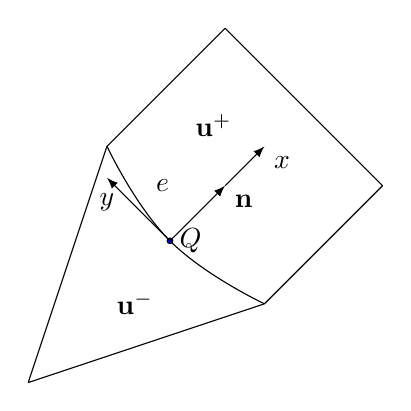
\begin{tikzpicture}[scale=1.0]
    \draw
    (0,0) -- (3,1)
    (1,3) -- (0,0)
    (3,1) -- (4.5,2.5)
    (4.5,2.5) -- (2.5,4.5)
    (2.5,4.5) -- (1,3);

    \draw plot [smooth,tension=0.8] coordinates { (3,1) (1.8,1.8) (1,3) };

    \draw[fill=blue,draw=black]
    (1,1) node[right]{$\mathbf{u}^{-}$}
    (1.5,2.5) node[right]{$e$}
    (2,3) node[above right]{$\mathbf{u}^{+}$}
    (1.8,1.8) circle (1pt) node[right]{$Q$};

    \draw[-latex] (1.8,1.8) -- (2.5,2.5) node[below right]{$\mathbf{n}$};
    \draw[-latex] (2.5,2.5) -- (3,3) node[below right]{$x$};
    \draw[-latex] (1.8,1.8) -- (1,2.6) node[below=2pt]{$y$};
    \end{tikzpicture}
\end{figure}
To guarantee the formal accuracy of the scheme, the numerical flux is required to satisfy the consistency relations
\begin{equation}
  \label{eq:10}
  \mathbf{h}_{\mathrm{e}}(\mathbf{u}^{-},\mathbf{u}^{+};\mathbf{n})=\mathbf{F}_{\mathrm{e}}(\mathbf{u})\cdot\mathbf{n},\quad\mathbf{h}_{\mathrm{e}}(\mathbf{u}^{-},\mathbf{u}^{+};\mathbf{n})=-\mathbf{h}_{\mathrm{e}}(\mathbf{u}^{-},\mathbf{u}^{+};-\mathbf{n}),
\end{equation}
Several numerical flux functions satisfy the above criteria such as the Godunov, Lax-Friedrichs, Roe, Engquist-Osher, or HLLE (Harten, Lax, Van Leer, Einfeldt).

The spatial discretization of the viscous term of the Navier-Stokes equations is constructed by resorting to a mixed finite element formulation. The first-order derivatives of the conservative variables appearing in the \autoref{eq:3} lead to second-order derivatives when we evaluate the divergence of the viscous fluxes. However, second-order derivatives cannot be accommodated directly in a weak variational formulation using a discontinuous function space. We therefore regard the gradient of the conservative variables $\mathbf{w}(\mathbf{u})=\nabla\mathbf{u}$ as auxiliary unknowns of the Navier-Stokes equations, which are therefore reformulated as the following coupled system for the unknowns $\mathbf{w}$ and $\mathbf{u}$,
\begin{equation}
  \label{eq:11}
  \begin{aligned}
    &\mathbf{w}-\nabla\mathbf{u}=0\\
    &\mathbf{u}_{,t}+\nabla\cdot\mathbf{F}_{\mathrm{e}}(\mathbf{u})-\nabla\cdot\mathbf{F}_{\mathrm{v}}(\mathbf{u},\mathbf{w})=\mathbf{S}(\mathbf{u},\mathbf{w}).
  \end{aligned}
\end{equation}

\autoref{eq:11} can be approximated using a discontinuous finite element formulation in a way similar to that employed for the inviscid part of the equations. The use of an explicit time-stepping scheme greatly simplifies the mixed finite element formulation, since it allows a decoupled solution of \autoref{eq:11}. At each time level $n$, in fact, we first compute a discontinuous approximation of $\mathbf{w}^{n}$ by solving the first equation of the system and then use $\mathbf{u}^{n}$ and $\mathbf{w}^{n}$ to evaluate the inviscid and viscous fluxes of the second equation which is then advanced in time.

Here by replacing $\mathbf{F}$ to $f\mathbf{c}$ for a scalar function $f$ and vector field $\mathbf{c}$ in the \href{https://en.wikipedia.org/wiki/Divergence_theorem}{divergence theorem} with specific forms, we have
\begin{equation}
  \int_{V}\mathbf{c}\cdot\nabla f\mathrm{d}V=\oint_{S}(\mathbf{c}f)\cdot\mathbf{n}\mathrm{d}S-\int_{V}f(\nabla\cdot\mathbf{c})\mathrm{d}V.
\end{equation}
The last term on the right vanishes for constant $\mathbf{c}$ or any divergence-free (solenoidal) vector field, e.g. Incompressible flows without sources or sinks such as phase change or chemical reactions etc. In particular, taking
$\mathbf{c}$ to be constant:
\begin{equation}
  \int_{V}\nabla f\mathrm{d}V=\oint_{S}f\mathbf{n}\mathrm{d}S
\end{equation}
Here, if the formula is rewritten into vector form, we have
\begin{equation}
  \int_{V}\nabla\mathbf{f}\mathrm{d}V=\oint_{S}\mathbf{f}\otimes\mathbf{n}\mathrm{d}S
\end{equation}

The weak formulation of the first equation of \autoref{eq:11} is
\begin{equation}
  \label{eq:15}
  \int_{E}\phi_{i}^{k}\mathbf{w}_{h}\mathrm{d}\Omega-\oint_{\partial E}\phi_{i}^{k}\mathbf{u}_{h}\otimes\mathbf{n}\mathrm{d}\sigma+\int_{E}\nabla\phi_{i}^{k}\otimes\mathbf{u}_{h}\mathrm{d}\Omega=0\quad 1\leqslant i\leqslant N_{k},
\end{equation}
where, due to the discontinuous function approximation at internal interfaces, the unknown $\mathbf{u}_{h}$ appearing in the boundary integral is not uniquely defined. In analogy with the procedure described for the inviscid part of the equations, it is therefore necessary to introduce a numerical flux function $\mathbf{h}_{\mathrm{w}}(\mathbf{u}^{-},\mathbf{u}^{+};\mathbf{n})$ to replace the term $\mathbf{u}_{h}\otimes\mathbf{n}$. Since we are constructing the discrete analog of a diffusive operator, we define the numerical flux function as the average between the two interface states, i.e., as
\begin{equation}
  \label{eq:16}
  \mathbf{h}_{\mathrm{w}}(\mathbf{u}^{-},\mathbf{u}^{+};\mathbf{n})=\dfrac{1}{2}(\mathbf{u}^{-}+\mathbf{u}^{+})\otimes\mathbf{n}.
\end{equation}

Here, unlike Bassi, we do not assemble all the mass matrices, but solve \autoref{eq:15} separately on each element $E$. The computed auxiliary variables $\mathbf{w}_{h}$ are then used in the weak form of the second equation of \autoref{eq:11},
\begin{equation}
  \label{eq:17}
  \begin{aligned}
    \int_{E}\phi_{i}^{k}\mathbf{u}_{h,t}\mathrm{d}\Omega &+\oint_{\partial E}\phi_{i}^{k}(\mathbf{F}_{\mathrm{e}}(\mathbf{u}_{h})+\mathbf{F}_{\mathrm{v}}(\mathbf{u}_{h},\mathbf{w}_{h}))\cdot\mathbf{n}\mathrm{d}\sigma\\
    &-\int_{E}\nabla\phi_{i}^{k}\cdot(\mathbf{F}_{\mathrm{e}}(\mathbf{u}_{h})+\mathbf{F}_{\mathrm{v}}(\mathbf{u}_{h},\mathbf{w}_{h}))\mathrm{d}\Omega=\int_{E}\phi_{i}^{k}\mathbf{S}(\mathbf{u}_{h},\mathbf{w}_{h})\mathrm{d}\Omega\quad 1\leqslant i\leqslant N_{k},
  \end{aligned}
\end{equation}
in which, once again, the boundary integral contains flux terms that are not uniquely defined. It is therefore necessary to replace the term $\mathbf{F}_{\mathrm{v}}(\mathbf{u}_{h},\mathbf{w}_{h})$ with the numerical flux function $\mathbf{h}_{\mathrm{v}}(\mathbf{u}^{-},\mathbf{w}^{-},\mathbf{u}^{+},\mathbf{w}^{+};\mathbf{n})$, defined in a ``centered'' way as
\begin{equation}
  \mathbf{h}_{\mathrm{v}}(\mathbf{u}^{-},\mathbf{w}^{-},\mathbf{u}^{+},\mathbf{w}^{+};\mathbf{n})=\dfrac{1}{2}(\mathbf{F}_{\mathrm{v}}(\mathbf{u}^{-},\mathbf{w}^{-})+\mathbf{F}_{\mathrm{v}}(\mathbf{u}^{+},\mathbf{w}^{+}))\cdot\mathbf{n}
\end{equation}

For there, an important issue in mixed finite element formulations is the choice of the approximation space for the auxiliary variables $\mathbf{w}_{h}$ concerning the original ones, i.e., the conservative variables $\mathbf{u}_{h}$. An inconsistent choice of the two approximation spaces may result in a solution that is polluted by spurious modes. We have not tried to address this issue from a theoretical point of view. In practice, we have used the same type of approximations for both $\mathbf{u}_{h}$ and $\mathbf{w}_{h}$. It is important to point out that, even if both $\mathbf{u}_{h}$ and $\mathbf{w}_{h}$ have been chosen in the same function space (say that of piecewise discontinuous polynomial $\mathbb{P}^{k}$ of order k inside each element), the auxiliary variable $\mathbf{w}_{h}$ can, however, be regarded as the sum of an ``interface contribution'' $\mathbf{w}_{h}^{\mathrm{int}}\in\mathbb{P}^{k}$ plus a ``volume contribution'' $\mathbf{w}_{h}^{\mathrm{vol}}\in\mathbb{P}^{k-1}$. Since $\mathbf{w}_{h}^{\mathrm{int}}$ vanishes when the jump of $\mathbf{u}_{h}$ at the element interfaces is zero, the auxiliary variable $\mathbf{w}_{h}\in\mathbb{P}^{k-1}$ when the solution $\mathbf{u}_{h}\in\mathbb{P}^{k}$ is continuous. In bassi's later papers, he will write $\mathbf{w}_{h}^{\mathrm{vol}}$ as $\nabla\mathbf{u}$ and $\mathbf{w}_{h}^{\mathrm{int}}$ as $\mathbf{r}$, that is to say, there are $\mathbf{w}=\nabla\mathbf{u}+\mathbf{r}$. Here we use the original notation. Next, let's introduce the BR1 format first.

In order to define $\mathbf{w}_{h}^{\mathrm{int}}$ and $\mathbf{w}_{h}^{\mathrm{vol}}$, it is necessary to rewrite the numerical flux function in \autoref{eq:16} as $\mathbf{u}+(\mathbf{u}^{+}-\mathbf{u}^{-})/2$ (here $\mathbf{u}$ is the same as $\mathbf{u}^{-}$). By inserting this expression into the boundary integral of \autoref{eq:15}, we obtain
\begin{equation}
  \label{eq:19}
  \int_{E}\phi_{i}^{k}\mathbf{w}_{h}\mathrm{d}\Omega=\oint_{\partial E}\phi_{i}^{k}\mathbf{u}_{h}\otimes\mathbf{n}\mathrm{d}\sigma+\oint_{\partial E}\phi_{i}^{k}\dfrac{1}{2}(\mathbf{u}_{h}^{+}-\mathbf{u}_{h}^{-})\otimes\mathbf{n}\mathrm{d}\sigma-\int_{E}\nabla\phi_{i}^{k}\otimes\mathbf{u}_{h}\mathrm{d}\Omega.
\end{equation}

Besides, the first and the last integrals appearing on the right-hand side of \autoref{eq:19} can be (back) integrated by parts to obtain a single volume integral, i.e.,
\begin{equation}
  \oint_{\partial E}\phi_{i}^{k}\mathbf{u}_{h}\otimes\mathbf{n}\mathrm{d}\sigma-\int_{E}\nabla\phi_{i}^{k}\otimes\mathbf{u}_{h}\mathrm{d}\Omega=\int_{E}\phi_{i}^{k}\nabla\mathbf{u}_{h}\mathrm{d}\Omega.
\end{equation}

\autoref{eq:19} can therefore be rewritten as
\begin{equation}
  \label{eq:21}
  \int_{E}\phi_{i}^{k}\mathbf{w}_{h}\mathrm{d}\Omega=\oint_{\partial E}\phi_{i}^{k}\dfrac{1}{2}(\mathbf{u}_{h}^{+}-\mathbf{u}_{h}^{-})\otimes\mathbf{n}\mathrm{d}\sigma+\int_{E}\phi_{i}^{k}\nabla\mathbf{u}_{h}\mathrm{d}\Omega.
\end{equation}

The contributions $\mathbf{w}_{h}^{\mathrm{int}}$ and $\mathbf{w}_{h}^{\mathrm{vol}}$ are given by the boundary and by the volume integrals appearing on the right-hand side of \autoref{eq:21}, i.e.,
\begin{equation}
  \label{eq:22}
  \int_{E}\phi_{i}^{k}\mathbf{w}_{h}^{\mathrm{int}}\mathrm{d}\Omega=\oint_{\partial E}\phi_{i}^{k}\dfrac{1}{2}(\mathbf{u}_{h}^{+}-\mathbf{u}_{h}^{-})\otimes\mathbf{n}\mathrm{d}\sigma,\quad \int_{E}\phi_{i}^{k}\mathbf{w}_{h}^{\mathrm{vol}}\mathrm{d}\Omega=\int_{E}\phi_{i}^{k}\nabla\mathbf{u}_{h}\mathrm{d}\Omega.
\end{equation}
We denote the numerical flux function in \autoref{eq:16} as $\mathbf{h}_{\mathrm{w}}^{\mathrm{vol}}(\mathbf{u}^{-},\mathbf{u}^{+};\mathbf{n})$, and similarly, we introduce a numerical flux function $\mathbf{h}_{\mathrm{w}}^{\mathrm{int}}(\mathbf{u}^{-},\mathbf{u}^{+};\mathbf{n})$ in the boundary integral here, which is defined as
\begin{equation}
  \mathbf{h}_{\mathrm{w}}^{\mathrm{int}}(\mathbf{u}^{-},\mathbf{u}^{+};\mathbf{n})=\dfrac{1}{2}(\mathbf{u}^{+}-\mathbf{u}^{-})\otimes\mathbf{n}.
\end{equation}
Please note that in some papers, the average value of the left and right states at the element boundary is denoted as $\{\mathbf{u}\}$, defined as $\{\mathbf{u}\}=(\mathbf{u}^{+}+\mathbf{u}^{-})/2$. With this notation, the first equation in \autoref{eq:22} will become:
\begin{equation}
  \int_{E}\phi_{i}^{k}\mathbf{w}_{h}^{\mathrm{int}}\mathrm{d}\Omega=\oint_{\partial E}\phi_{i}^{k}(\{\mathbf{u}_{h}\}-\mathbf{u}_{h})\otimes\mathbf{n}\mathrm{d}\sigma
\end{equation}
These two equations only differ in notation, but they are equivalent. So for the formulation of BR1, the \autoref{eq:17} can be rewritten as
\begin{equation}
  \label{eq:24}
  \begin{aligned}
    \int_{E}\phi_{i}^{k}\mathbf{u}_{h,t}\mathrm{d}\Omega &+\oint_{\partial E}\phi_{i}^{k}(\mathbf{F}_{\mathrm{e}}(\mathbf{u}_{h})\cdot\mathbf{n}+\mathbf{F}_{\mathrm{v}}(\mathbf{u}_{h},\mathbf{w}_{h}^{\mathrm{int}}+\mathbf{w}_{h}^{\mathrm{vol}})\cdot\mathbf{n})\mathrm{d}\sigma\\
    &-\int_{E}\nabla\phi_{i}^{k}\cdot(\mathbf{F}_{\mathrm{e}}(\mathbf{u}_{h})+\mathbf{F}_{\mathrm{v}}(\mathbf{u}_{h},\mathbf{w}_{h}^{\mathrm{int}}+\mathbf{w}_{h}^{\mathrm{vol}}))\mathrm{d}\Omega=\int_{E}\phi_{i}^{k}\mathbf{S}(\mathbf{u}_{h},\mathbf{w}_{h}^{\mathrm{int}}+\mathbf{w}_{h}^{\mathrm{vol}})\mathrm{d}\Omega\quad 1\leqslant i\leqslant N_{k}.
  \end{aligned}
\end{equation}
Unfortunately, this formulation can be shown to be singular in some model problems and displays an unsatisfactory convergence rate for polynomial approximations of odd order.

A cure to this problem, which is BR2 format, has been found by replacing the $\mathbf{w}_{h}^{\mathrm{int}}$ in the contour integral of \autoref{eq:24} with ``face'' contributions redefined as
\begin{equation}
  \int_{E}\phi_{i}^{k}\mathbf{w}_{h|e}^{\mathrm{int}}\mathrm{d}\Omega=\int_{e}\phi_{i}^{k}\dfrac{1}{2}(\mathbf{u}_{h}^{+}-\mathbf{u}_{h}^{-})\otimes\mathbf{n}\mathrm{d}\sigma\quad\forall e \in\partial E.
\end{equation}
Notice that the following relation between the functions $\mathbf{w}_{h}^{\mathrm{int}}$ and $\mathbf{w}_{h|e}^{\mathrm{int}}$ holds
\begin{equation}
  \mathbf{w}_{h}^{\mathrm{int}}=\sum_{e\in\partial E}\mathbf{w}_{h|e}^{\mathrm{int}}.
\end{equation}
With this modification, \autoref{eq:24} becomes
\begin{equation}
  \label{eq:27}
  \begin{aligned}
    \int_{E}\phi_{i}^{k}\mathbf{u}_{h,t}\mathrm{d}\Omega &+\oint_{\partial E}\phi_{i}^{k}(\mathbf{F}_{\mathrm{e}}(\mathbf{u}_{h})\cdot\mathbf{n}+\mathbf{F}_{\mathrm{v}}(\mathbf{u}_{h},\eta_{e}\mathbf{w}_{h|e}^{\mathrm{int}}+\mathbf{w}_{h}^{\mathrm{vol}})\cdot\mathbf{n})\mathrm{d}\sigma\\
    &-\int_{E}\nabla\phi_{i}^{k}\cdot(\mathbf{F}_{\mathrm{e}}(\mathbf{u}_{h})+\mathbf{F}_{\mathrm{v}}(\mathbf{u}_{h},\mathbf{w}_{h}^{\mathrm{int}}+\mathbf{w}_{h}^{\mathrm{vol}}))\mathrm{d}\Omega=\int_{E}\phi_{i}^{k}\mathbf{S}(\mathbf{u}_{h},\mathbf{w}_{h}^{\mathrm{int}}+\mathbf{w}_{h}^{\mathrm{vol}})\mathrm{d}\Omega\quad 1\leqslant i\leqslant N_{k}.
  \end{aligned}
\end{equation}
In the formula, $\eta_{e}$ is the stability factor, which is usually taken as the number of interfaces of the element\cite{bassiImplicitHighorderDiscontinuous2007}. In some articles, this value is also directly set to $3.0$, but numerical experiments here show that setting it to $1.0$ is sufficient for stability.

\section{Basis Functions}

For the basis functions, the only requirement here is to satisfy completeness on each element, meaning they must be able to span the function space $\mathbb{V}_{h}^{k}$,
\begin{equation}
  \mathbb{V}_{h}^{k}:=\{\phi^{k}\in L^{2}(\Omega_{h}):\phi^{k}_{|E}\in\mathbb{P}^{k},\quad\forall E\in\mathscr{E}_{h}\},
\end{equation}
Under this condition, any set of basis functions that can span this space can be used as basis functions. Examples include Lagrange basis functions, Gauss-Lobatto-Legendre basis functions, Taylor basis functions, and Legendre basis functions. These basis functions can be classified into two categories: nodal basis functions and modal basis functions.

Nodal basis functions are constructed by interpolating based on nodal values within an element, allowing for the rapid retrieval of values at predefined nodes within the element. Different interpolation nodes lead to different basis functions. For instance, the \href{https://docs.fenicsproject.org/dolfinx/main/python/demos/demo_lagrange_variants.html}{Gauss-Lobatto-Legendre} basis functions are constructed using Gauss-Lobatto quadrature points as interpolation nodes. This enables quick evaluation of values at quadrature points within the element. Additionally, since values at interpolation nodes can be obtained, nodal basis functions facilitate h-adaptive methods or DG/FV hybrid methods.

Modal basis functions are generally composed of a hierarchical set of basis functions, and orthogonality is not inherently required. For example, Taylor basis functions do not require orthogonality. Besides, basis functions can be orthogonalized, as in the case of Legendre basis functions. In some implicit methods, this orthogonalization can lead to a stiffness matrix with a better condition number. However, in practice, implicit methods are often paired with preconditioning techniques to reduce the condition number of the matrix.It is important to note that this orthogonalization is only valid on the reference element. High-order curved mesh transformations can break this orthogonality. The hierarchical nature of modal basis functions means that a basis function of order $p+1$ inherently contains the basis functions of order $p$. This property is particularly useful in certain shock-capturing schemes. Furthermore, it allows for cross-order initialization, making modal basis functions well-suited for p-adaptive methods.

The implementation of basis functions here is primarily based on \href{https://gmsh.info}{gmsh}. For nodal basis functions, we directly use Lagrange basis functions for post-processing and output. For modal basis functions, we use the H1Legendre basis functions provided in gmsh, which are essentially Lobatto basis functions \cite{solinHigherOrderFiniteElement2003}. Compared to Legendre basis functions, Lobatto basis functions offer better matrix conditioning. In our computations, we consistently use Lobatto basis functions. Here Lagrange basis functions are defined as
\begin{equation}
  \phi_{i}^{k}=\prod_{j=1,j\neq i}^{N_{k}}\dfrac{f_{j}(\xi,\eta,\zeta)}{f_{j}(\xi_{i},\eta_{i},\zeta_{i})},\quad 1\leqslant i\leqslant N_{k}.
\end{equation}
The Lagrange basis functions have the following properties
\begin{equation}
  \phi_{i}^{k}(\xi_{j},\eta_{j},\zeta_{j})=\delta_{ij},\quad \sum_{i=1}^{N_{k}}\phi_{i}^{k}(\xi,\eta,\zeta)=1.
\end{equation}
Therefore, we can also construct basis functions by using the undetermined coefficient method for complete polynomials.

% For a two-dimensional triangular element, its reference element in gmsh is defined as

% \begin{figure}[H]
%   \centering
%   \includegraphics[width=1.00\textwidth]{figures/tri-reference.pdf}
% \end{figure}

% From left to right, the reference element of order 1, order 2, and order 3 and the distribution of corresponding Lagrange interpolation points. The shape of the $\phi_{3}^{2}$ and $\phi_{4}^{2}$ of the second-order element are shown here

% \begin{figure}[H]
%   \centering
%   \includegraphics[width=1.00\textwidth]{figures/tri-basis-fun.pdf}
% \end{figure}

% For a two-dimensional quadrangle element, its reference element in gmsh is defined as

% \begin{figure}[H]
%   \centering
%   \includegraphics[width=1.00\textwidth]{figures/quad-reference.pdf}
% \end{figure}

% From left to right, the reference element of order 1, order 2, and order 3 and the distribution of corresponding Lagrange interpolation points. The shape of the $\phi_{4}^{2}$ and $\phi_{5}^{2}$ of the second-order element are shown here

% \begin{figure}[H]
%   \centering
%   \includegraphics[width=1.00\textwidth]{figures/quad-basis-fun.pdf}
% \end{figure}

For the Lagrange basis functions, it is easy to construct their interpolation functions, and we can convert straight-line elements to isoparametric elements by coordinate transformation. However, this type of element has certain disadvantages, mainly because of the internal nodes that increase with the increase of the interpolation function, thereby increasing the number of degrees of freedom of the element. The addition of these degrees of freedom usually does not improve the accuracy of the element, because the accuracy of the element is usually determined by the power of a complete polynomial. Therefore, if you use Taylor basis functions for computation, they only include the orders of complete polynomials. This allows achieving the required accuracy with minimal computational cost. This is why some literature prefers Taylor basis functions over Lagrange basis functions.

\section{Curved Mesh}

For the FVM (Finite Volume Method), we generally seldom consider curved mesh. This is because FVM itself is either cell-centered or vertex-centered, and it is insensitive to grid deformation. However, for the DG (Discontinuous Galerkin) method, we need to consider curved mesh because the discrete solution in DG is approximated by high-order polynomials on elements, and the coefficients of these polynomials need to be integrated over the elements. Therefore, we need to consider the influence of grid deformation on integration, which Bassi also described in detail in his paper\cite{bassiHighOrderAccurateDiscontinuous1997}.

As the isoparametric element is used here, which means that the interpolation functions for the coordinates transformation of the element's geometry use the same interpolation basis functions and interpolation nodes as those used to describe the displacement modes of the element, we have
\begin{equation}
  \mathbf{x}(\xi,\eta,\zeta)=\sum_{i=1}^{N_{k}}\phi_{i}^{k}(\xi,\eta,\zeta)\mathbf{x}_{i}.
\end{equation}
The element transformation is as follows:
\begin{figure}[H]
  \centering
  \begin{tikzpicture}[scale=1.0]
    \draw[fill=blue,draw=black]
    (0,0) circle (1pt) node[below]{$\xi_1$}
    (3,0) circle (1pt) node[below]{$\xi_2$}
    (0,3) circle (1pt) node[above right]{$\xi_3$}
    (1.5,0) circle (1pt) node[below]{$\xi_4$}
    (1.5,1.5) circle (1pt) node[above right]{$\xi_5$}
    (0,1.5) circle (1pt) node[above left]{$\xi_6$};

    \draw (0,3) -- (3,0);
    \draw[-latex] (0,0) -- (4,0) node[right]{$\xi$};
    \draw[-latex] (0,0) -- (0,4) node[right]{$\eta$};

    \draw[fill=blue,draw=black]
    (7,1) circle (1pt) node[below]{$x_1$}
    (10,3) circle (1pt) node[below]{$x_2$}
    (7,5) circle (1pt) node[above right]{$x_3$}
    (8,2) circle (1pt) node[above left]{$x_4$}
    (9,4) circle (1pt) node[above right]{$x_5$}
    (6,3) circle (1pt) node[left]{$x_6$};

    \draw plot [smooth,tension=0.8] coordinates { (7,1) (8,2) (10,3) };
    \draw plot [smooth,tension=0.8] coordinates { (10,3) (9,4) (7,5) };
    \draw plot [smooth,tension=0.8] coordinates { (7,5) (6,3) (7,1) };
    \draw[-latex] (8,0) -- (9,0) node[right]{$x$};
    \draw[-latex] (8,0) -- (8,1) node[right]{$y$};

    \draw (3,3) node[below right]{$\mathbf{x}(\xi,\eta)$};
    \draw[-latex] plot [smooth,tension=0.8] coordinates { (0.5,1.5) (3,3) (7,4) };
    \end{tikzpicture}
\end{figure}
Therefore, we can use this formula to calculate the Jacobi matrix $[\mathbf{J}]$ and its transpose inverse matrix $[\mathbf{J}]^{-\mathrm{T}}$. The Jacobian matrix $[\mathbf{J}]$ can be obtained by the following formula:
\begin{equation}
  [\mathbf{J}](\xi,\eta,\zeta)=\dfrac{\partial(x,y,z)}{\partial(\xi,\eta,\zeta)}=\hat{\nabla}\mathbf{x}(\xi,\eta,\zeta)=\sum_{i=1}^{N_{k}}\hat{\nabla}\phi_{i}^{k}(\xi,\eta,\zeta)\mathbf{x}_{i},
\end{equation}
and $\hat{\nabla}$ is the gradient operator in the reference element. In the program, we directly use gmsh's API to obtain the derivative values of the basis functions concerning the reference element and the inverse matrix of the Jacobian for each element.

Next, let's discuss how to compute the derivatives of the basis functions at each element. This is necessary as they appear in the volume integration. Obtaining the derivatives of the basis functions concerning the local coordinates is straightforward since they are polynomials. However, what we need are the derivatives of the basis functions concerning the global coordinates, as we require them for computing the volume integration in the global coordinate system. To achieve this, we need to apply the chain rule, i.e.,
\begin{equation}
  \dfrac{\partial\phi_{i}^{k}}{\partial x_{j}}=\dfrac{\partial\phi_{i}^{k}}{\partial\xi}\dfrac{\partial\xi}{\partial x_{j}}+\dfrac{\partial\phi_{i}^{k}}{\partial\eta}\dfrac{\partial\eta}{\partial x_{j}}+\dfrac{\partial\phi_{i}^{k}}{\partial\zeta}\dfrac{\partial\zeta}{\partial x_{j}},
\end{equation}
which can be written in matrix form as
\begin{equation}
  \nabla\phi_{i}^{k}(\xi,\eta,\zeta)=\begin{bNiceMatrix}
    \dfrac{\partial\phi_{i}^{k}}{\partial x}\\
    \dfrac{\partial\phi_{i}^{k}}{\partial y}\\
    \dfrac{\partial\phi_{i}^{k}}{\partial z}
  \end{bNiceMatrix}=\begin{bNiceMatrix}
    \dfrac{\partial\xi}{\partial x}&\dfrac{\partial\eta}{\partial x}&\dfrac{\partial\zeta}{\partial x}\\
    \dfrac{\partial\xi}{\partial y}&\dfrac{\partial\eta}{\partial y}&\dfrac{\partial\zeta}{\partial y}\\
    \dfrac{\partial\xi}{\partial z}&\dfrac{\partial\eta}{\partial z}&\dfrac{\partial\zeta}{\partial z}
  \end{bNiceMatrix}\begin{bNiceMatrix}
    \dfrac{\partial\phi_{i}^{k}}{\partial\xi}\\
    \dfrac{\partial\phi_{i}^{k}}{\partial\eta}\\
    \dfrac{\partial\phi_{i}^{k}}{\partial\zeta}
  \end{bNiceMatrix}=[\mathbf{J}]^{-\mathrm{T}}\cdot\hat{\nabla}\phi_{i}^{k}(\xi,\eta,\zeta).
\end{equation}
Then, we calculate the derivative values of the basis functions concerning the actual element. The \autoref{eq:9} in reference element $\hat{E}$ can be written as
\begin{equation}
  \label{eq:35}
  \begin{aligned}
    \int_{\hat{E}}\phi_{i}^{k}\mathbf{u}_{h,t}|\mathbf{J}|\mathrm{d}\hat{\Omega} &+\oint_{\partial \hat{E}}\phi_{i}^{k}\mathbf{F}(\mathbf{u}_{h},\nabla\mathbf{u}_{h})\cdot\mathbf{n}|\mathbf{J}|\mathrm{d}\hat{\sigma}\\
    &-\int_{\hat{E}}\left([\mathbf{J}]^{-\mathrm{T}}\cdot\hat{\nabla}\phi_{i}^{k}\right)\cdot\mathbf{F}(\mathbf{u}_{h},\nabla\mathbf{u}_{h})|\mathbf{J}|\mathrm{d}\hat{\Omega}=\int_{\hat{E}}\phi_{i}^{k}\mathbf{S}(\mathbf{u}_{h},\nabla\mathbf{u}_{h})|\mathbf{J}|\mathrm{d}\hat{\Omega}\quad 1\leqslant i\leqslant N_{k}.
  \end{aligned}
\end{equation}

We introduce how to solve for the normal vector on the boundary of the isoparametric element. First, let's consider the two-dimensional case, which involves finding the normal vector to a two-dimensional curve at its boundary. Here, the tangent vector to the two-dimensional curve can be directly obtained. The normal vector can be obtained by rotating the tangent vector by $90^{\circ}$. Specifically,
\begin{equation}
  \bm{\tau}=\begin{bNiceMatrix}
    \dfrac{\partial x}{\partial \xi}\\
    \dfrac{\partial y}{\partial \xi}
  \end{bNiceMatrix}=\begin{bNiceMatrix}
    \displaystyle\sum_{i=1}^{N_{k}}\dfrac{\partial\phi_{i}^{k}}{\partial \xi}x_{i}\\
    \displaystyle\sum_{i=1}^{N_{k}}\dfrac{\partial\phi_{i}^{k}}{\partial \xi}y_{i}
  \end{bNiceMatrix},\mathbf{n}=\mathbf{M}\left(-\dfrac{\pi}{2}\right)\bm{\tau}=\begin{bNiceMatrix}
    0&1\\
    -1&0
  \end{bNiceMatrix}\begin{bNiceMatrix}
    \dfrac{\partial x}{\partial \xi}\\
    \dfrac{\partial y}{\partial \xi}
  \end{bNiceMatrix}=\begin{bNiceMatrix}
    \displaystyle\sum_{i=1}^{N_{k}}\dfrac{\partial\phi_{i}^{k}}{\partial \xi}y_{i}\\
    \displaystyle-\sum_{i=1}^{N_{k}}\dfrac{\partial\phi_{i}^{k}}{\partial \xi}x_{i}
  \end{bNiceMatrix}.
\end{equation}
Next, let's consider the three-dimensional case, where we need to find the normal vector to a three-dimensional surface. Here, we seek two tangent vectors of the three-dimensional surface in the tangent plane and then obtain the normal vector by taking the cross-product of these two tangent vectors. Define $\mathbf{r}=(x(\xi,\eta),y(\xi,\eta),z(\xi,\eta))$, then
\begin{equation}
  \begin{aligned}
    \bm{\tau}_{\xi}&=\dfrac{\partial\mathbf{r}}{\partial\xi}=\begin{bNiceMatrix}
      \dfrac{\partial x}{\partial\xi}\\
      \dfrac{\partial y}{\partial\xi}\\
      \dfrac{\partial z}{\partial\xi}
    \end{bNiceMatrix},\quad\bm{\tau}_{\eta}=\dfrac{\partial\mathbf{r}}{\partial\eta}=\begin{bNiceMatrix}
      \dfrac{\partial x}{\partial\eta}\\
      \dfrac{\partial y}{\partial\eta}\\
      \dfrac{\partial z}{\partial\eta}
    \end{bNiceMatrix}\\
    \mathbf{n}&=\bm{\tau}_{\xi}\times\bm{\tau}_{\eta}=\begin{bNiceMatrix}
      \dfrac{\partial x}{\partial\xi}\\
      \dfrac{\partial y}{\partial\xi}\\
      \dfrac{\partial z}{\partial\xi}
    \end{bNiceMatrix}\times\begin{bNiceMatrix}
      \dfrac{\partial x}{\partial\eta}\\
      \dfrac{\partial y}{\partial\eta}\\
      \dfrac{\partial z}{\partial\eta}
    \end{bNiceMatrix}=\begin{bNiceMatrix}
      \displaystyle\sum_{i=1}^{N_{k}}\dfrac{\partial\phi_{i}^{k}}{\partial \xi}x_{i}\\
      \displaystyle\sum_{i=1}^{N_{k}}\dfrac{\partial\phi_{i}^{k}}{\partial \xi}y_{i}\\
      \displaystyle\sum_{i=1}^{N_{k}}\dfrac{\partial\phi_{i}^{k}}{\partial \xi}z_{i}
    \end{bNiceMatrix}\times\begin{bNiceMatrix}
      \displaystyle\sum_{i=1}^{N_{k}}\dfrac{\partial\phi_{i}^{k}}{\partial \eta}x_{i}\\
      \displaystyle\sum_{i=1}^{N_{k}}\dfrac{\partial\phi_{i}^{k}}{\partial \eta}y_{i}\\
      \displaystyle\sum_{i=1}^{N_{k}}\dfrac{\partial\phi_{i}^{k}}{\partial \eta}z_{i}
    \end{bNiceMatrix}.
  \end{aligned}
\end{equation}

\section{Numerical Integral}

For the integrals in \autoref{eq:35}, both on the elements and at element edges, numerical integration is typically employed, such as Gauss quadrature. Cockburn's paper\cite{cockburnRungeKuttaLocalProjection1990} provides the order requirements for Gauss quadrature for different integrals in this context. Here's a direct excerpt from the original text: \textit{Assume that the family of triangulations $\mathscr{F}$ is regular and \textbf{B}-uniform. Suppose that $V(K)\supset P^{k}(K)$, $\forall K\in\mathscr{T}_{h}$, $\forall\mathscr{T}_{h}\in\mathscr{F}$, and that the quadrature rule over the edges is exact for polynomials of degree $(2k +1)$, and the quadrature rule over the elements is exact for polynomials of degree $2k$. Then:}
\begin{enumerate}
  \item \textit{The RKDG method is formally uniformly $(k+1)$st-order accurate in time and space if $\Delta t=\mathcal{O}(h)$};
  \item \textit{The approximate solution generated by the RKDG method verifies the maximum principle $(2.8)$ if the CFL-condition $(2.19)$ is verified with $\delta=\mathrm{max}_{i,l}\left|\frac{\beta_{i,l}}{\alpha_{i,l}}\right|$};
  \item \textit{The approximate solution converges to a weak solution of $(1.1)$ if there is a constant $C$ such that $||\bar{u}_{h}||_{BV(\Omega)}\le C$};
\end{enumerate}

The discussion about Gauss quadrature is largely based on Solin\cite{solinHigherOrderFiniteElement2003}, and you can find tables of weights and integration points for different orders of Gaussian quadrature in the book. So let's start from the one-dimensional domain. The quadrature rules of the Gauss type are based on the summation of weighted function values on non-equidistantly distributed integration points. The $n$-point Gauss quadrature rule for the one-dimensional line reference domain $\hat{E}_{l}=(-1,1)$ reads
\begin{equation}
  \int_{-1}^{1}f(\xi)\mathrm{d}\xi\approx\sum_{i=1}^{n}w_{n,i}f(\xi_{n,i}).
\end{equation}
Analogously as for the Chebyshev and Lobatto (Radau) rules, the integration points and weights can be obtained after inserting sufficiently many linearly independent functions with known integrals and resolving the resulting system of nonlinear algebraic equations. Since we have $2n$ unknown parameters at our disposal ($n$ integration points $\xi_{n,i}$ and $n$ weights $w_{n,i}$), the resulting formula will be accurate for all polynomials of order $2n-1$ and lower.

It can be shown that the integration points are roots of the Legendre polynomials $L_{n}(\xi)$. Hence, the complexity of the problem reduces to the level of Newton-Cotes quadrature rules, since with known points the nonlinear system comes over to a system of linear algebraic equations. The analysis leads even further; it is known that the weights $w_{n,i}$ can be expressed as
\begin{equation}
  w_{n,i}=\dfrac{2}{(1-\xi_{n,i}^{2})[L_{n}'(\xi_{n,i})]^{2}}, \quad i=1,\dots,n.
\end{equation}
For two-dimensional Gaussian quadrature in the quadrilateral domain $\hat{E}_{q}$, let us start with a technique that is easiest to implement - quadrature formulae based on the Cartesian product of two one-dimensional quadrature rules in the axial directions $\xi_{1}$ and $\xi_{2}$. Consider the formula
\begin{equation}
  \int_{\hat{E}_{l}}f(\xi)\mathrm{d}\xi\approx\sum_{i=1}^{M_{a}}w_{g_{a},i}f(y_{g_{a},i}),
\end{equation}
where $y_{g_{a},i},w_{g_{a},i}$ are Gauss integration points and weights on the one-dimensional reference domain $\hat{E}_{l}=(-1,1)$ that integrate exactly all polynomials of the order $p$ and lower. It is easy to see that the product formula
\begin{equation}
  \int_{\hat{E}_{l}}g(\xi_{1},\xi_{2})\mathrm{d}\xi_{1}\mathrm{d}\xi_{2}\approx\sum_{i=1}^{M_{a}}\sum_{j=1}^{M_{a}}w_{g_{a},i}w_{g_{b},j}f(y_{g_{a},i},y_{g_{b},j})
\end{equation}
is of the order $p$ for polynomials of two independent variables $\xi_{1},\xi_{2}$. In addition to its simple implementation, the product formula has one more advantage - it can easily be generalized to polynomials with different orders of approximation in the axial directions $\xi_{1},\xi_{2}$. Such polynomials may appear naturally as a consequence of $p$-anisotropic refinements of quadrilateral elements, that may occur, e.g., within boundary and internal layers. However, the Gaussian quadrature formulas obtained in this way do not always use the minimum number of points. It is possible to achieve a more efficient Gaussian quadrature formula by eliminating some symmetric points while maintaining the original polynomial degree. We won't go into the specific details of this approach here, as it is not the one we have adopted.

However, for triangular elements, the situation is more complicated. The fundamental equation for the construction of the integration points and weights for the reference triangle $\hat{E}_{t}$ reads
\begin{equation}
  \int_{-1}^{1}\int_{-1}^{1-\xi_{1}}f(\xi_{1},\xi_{2})\mathrm{d}\xi_{2}\mathrm{d}\xi_{1}\approx\sum_{i=1}^{n}w_{i}f(\xi_{1,i},\xi_{2,i}),
\end{equation}
where $n$ denotes the number of integration points. Each point is characterized by three unknowns: $\omega_{i},\xi_{1,i}$ and $\xi_{2,i}$. If we want to solve for these three unknowns, we will need to solve a nonlinear system of algebraic equations. It is practically infeasible to calculate the integration points and weights for higher values of $p$ by standard methods or mathematical software. Lyness\cite{lynessModerateDegreeSymmetric1975} proposed a sophisticated algorithm based on determining the points and weights within an equilateral triangle in polar coordinates, taking advantage of its multiple symmetries. The algorithm provides the minimum number of Gaussian points for any polynomial order $p$ and strongly reduces the size of the nonlinear system. Dunavant\cite{dunavantHighDegreeEfficient1985} extended the algorithm and calculated the points and weights up to the order $p=20$ (some weights being negative and some points lying outside the triangle). The position of integration points and values of the weights corresponding to other triangles can be obtained by a simple affine transformation.

The fact that some of the weights are negative means that the stability of the quadrature will tend to decrease when integrating oscillatory functions whose polynomial behavior exceeds the order of accuracy of the quadrature formulae. In this case, the schemes still can be used, but one has to combine them with spatial refinements of the reference element. If oscillations (or other excessive nonlinearities) in the integrated functions are expected, an application of adaptive formulae that compare results from several refinement levels may be a good idea.

\section{Convective Flux}

We mentioned some methods for calculating convective numerical fluxes at \autoref{eq:10}, and here we will introduce these methods in some detail. Note that what our convective numerical flux needs to replace here is $\mathbf{F}_{\mathrm{e}}(\mathbf{u})\cdot\mathbf{n}$, which means that the flux we calculate is on the normal vector $\mathbf{n}$, which will cause a relatively large change compared to the one-dimensional form for some schemes. Here we focus on how to calculate these formats, and we will not introduce too much about the properties and derivation of these schemes.

Here we first define some symbols that we will use next. The first is the value on the left and right sides of the conserved variable $\mathbf{u}$. $\mathbf{u}^{-}$ represents the value on the left side of the interface, and $\mathbf{u}^{+}$ represents the value on the right side of the interface. $V=u n_{x}+v n_{y}+w n_{z}$ represents the velocity along the interface normal vector.
\begin{equation}
  \mathbf{F}_{\mathrm{e},n}=\mathbf{F}_{\mathrm{e}}\cdot\mathbf{n}=\mathbf{f}_{\mathrm{e}}n_{x}+\mathbf{g}_{\mathrm{e}}n_{y}+\mathbf{h}_{\mathrm{e}}n_{z}=\begin{bNiceMatrix}
    \rho(u n_{x}+v n_{y}+w n_{z})\\
    \rho u(u n_{x}+v n_{y}+w n_{z})+p n_{x}\\
    \rho v(u n_{x}+v n_{y}+w n_{z})+p n_{y}\\
    \rho w(u n_{x}+v n_{y}+w n_{z})+p n_{z}\\
    (u n_{x}+v n_{y}+w n_{z})(\rho E+p)
  \end{bNiceMatrix}=\begin{bNiceMatrix}
    \rho V\\
    \rho u V+p n_{x}\\
    \rho v V+p n_{y}\\
    \rho w V+p n_{z}\\
    V(\rho E+p)
  \end{bNiceMatrix}
\end{equation}

\subsection*{Lax-Friedrichs Scheme}

The Lax-Friedrichs scheme is the simplest, and it is also the most stable scheme. The Lax-Friedrichs scheme can be evaluated by the following formula
\begin{equation}
  \mathbf{h}_{\mathrm{e}}(\mathbf{u}^{-},\mathbf{u}^{+};\mathbf{n})=\dfrac{1}{2}(\mathbf{F}_{\mathrm{e},n}(\mathbf{u}^{-})+\mathbf{F}_{\mathrm{e},n}(\mathbf{u}^{+}))-\dfrac{1}{2}\alpha(\mathbf{u}^{+}-\mathbf{u}^{-}),
\end{equation}
where $\alpha$ is the maximum eigenvalue of the Jacobian matrix $\mathbf{A}_{\mathrm{e},n}(\mathbf{u})=\partial\mathbf{F}_{\mathrm{e},n}/\partial\mathbf{u}$ of the convective flux along the normal vector direction. The eigenvalues are
\begin{equation}
  \lambda_{1}=V-c,\quad\lambda_{2}=V,\quad\lambda_{3}=V,\quad\lambda_{4}=V,\quad\lambda_{5}=V+c.
\end{equation}

\subsection*{HLLC Scheme}

The derivation of the HLLC scheme is based on the book of Toro\cite{toroRiemannSolversNumerical2009a} and the paper of Batten et al.\cite{battenChoiceWavespeedsHLLC1997}. To determine completely the numerical fluxes in the HLLC scheme, we need to provide an algorithm for computing the wave speeds $S^{-}$, $S^{+}$ and $S^{*}$. The $S^{-}$ and $S^{+}$ are the speeds of the left and right waves, respectively, and $S^{*}$ is the speed of the contact wave. Here we use the pressure-based wave speed estimates proposed by Toro to calculate the wave speeds, whereby one first finds an estimate for the pressure $p^{*}$. For the estimate of the pressure, we use the ideal gases simplified PVRS approximate Riemann solver to calculate it.

Step one is to calculate the pressure $p^{*}$, which is given by
\begin{equation}
  p^{*}=\max(0, p_{\mathrm{pvrs}}),\quad p_{\mathrm{pvrs}}=\dfrac{1}{2}(p^{-}+p^{+})-\dfrac{1}{2}(V^{+}-V^{-})\bar{\rho}\bar{c},\quad\bar{\rho}=\dfrac{1}{2}(\rho^{-}+\rho^{+}),\quad\bar{c}=\dfrac{1}{2}(c^{-}+c^{+}).
\end{equation}

Step two is to calculate the wave speeds $S^{-}$, $S^{+}$ and $S^{*}$. The $S^{-}$ and $S^{+}$ are the speeds of the left and right waves, respectively, which are given by
\begin{equation}
  S^{-}=V^{-}-c^{-}q^{-},\quad S^{+}=V^{+}+c^{+}q^{+},\quad q^{\pm}=
  \begin{cases}
    1&\text{if }p^{*}\leqslant p^{\pm},\\
    \sqrt{1+\dfrac{\gamma+1}{2\gamma}\left(\dfrac{p^{*}}{p^{\pm}}-1\right)}&\text{if }p^{*}>p^{\pm}.
  \end{cases}
\end{equation}
Then the $S^{*}$ is the speed of the contact wave, which is given by
\begin{equation}
  S^{*}=\dfrac{p^{+}-p^{-}+\rho^{-}V^{-}(S^{-}-V^{-})-\rho^{+}V^{+}(S^{+}-V^{+})}{\rho^{-}(S^{-}-V^{-})-\rho^{+}(S^{+}-V^{+})}.
\end{equation}

Step three is to calculate the HLLC numerical fluxes. The HLLC numerical fluxes are given by
\begin{equation}
  \mathbf{h}_{\mathrm{e}}(\mathbf{u}^{-},\mathbf{u}^{+};\mathbf{n})=
  \begin{cases}
    \mathbf{F}_{\mathrm{e},n}(\mathbf{u}^{-})&\text{if }0\leqslant S^{-},\\
    \mathbf{F}_{\mathrm{e},n}(\mathbf{u}^{-})+S^{-}(\mathbf{u}^{*,-}-\mathbf{u}^{-})&\text{if }S^{-}\leqslant 0\leqslant S^{*},\\
    \mathbf{F}_{\mathrm{e},n}(\mathbf{u}^{+})+S^{+}(\mathbf{u}^{*,+}-\mathbf{u}^{+})&\text{if }S^{*}\leqslant 0\leqslant S^{+},\\
    \mathbf{F}_{\mathrm{e},n}(\mathbf{u}^{+})&\text{if }0\geqslant S^{+},
  \end{cases}
\end{equation}
where $\mathbf{u}^{*,-}$ and $\mathbf{u}^{*,+}$ are the intermediate states on the left and right sides of the interface, respectively, which are given by
\begin{equation}
  \mathbf{u}^{*,\pm}=\begin{bNiceMatrix}
    \rho^{\pm}\dfrac{S^{\pm}-V^{\pm}}{S^{\pm}-S^{*}}\\
    \dfrac{\rho^{\pm}V^{\pm}(S^{\pm}-V^{\pm})+(p^{*}-p^{\pm})n_{x}}{S^{\pm}-S^{*}}\\
    \dfrac{\rho^{\pm}V^{\pm}(S^{\pm}-V^{\pm})+(p^{*}-p^{\pm})n_{y}}{S^{\pm}-S^{*}}\\
    \dfrac{\rho^{\pm}V^{\pm}(S^{\pm}-V^{\pm})+(p^{*}-p^{\pm})n_{z}}{S^{\pm}-S^{*}}\\
    \dfrac{\rho^{\pm}E^{\pm}(S^{\pm}-V^{\pm})-p^{\pm}V^{\pm}+p^{*}S^{*}}{S^{\pm}-S^{*}}
  \end{bNiceMatrix}.
\end{equation}

\subsection*{Roe Scheme}

Most of the derivation of the Roe scheme here comes from the books of Blazek\cite{blazekComputationalFluidDynamics2015} and Toro\cite{toroRiemannSolversNumerical2009a}, and some of them are derived by myself. The Roe scheme can be evaluated by the following formula
\begin{equation}
  \begin{aligned}
    \mathbf{h}_{\mathrm{e}}(\mathbf{u}^{-},\mathbf{u}^{+};\mathbf{n})&=\dfrac{1}{2}(\mathbf{F}_{\mathrm{e},n}(\mathbf{u}^{-})+\mathbf{F}_{\mathrm{e},n}(\mathbf{u}^{+}))-\dfrac{1}{2}\tilde{\mathbf{A}}_{\mathrm{e}}(\mathbf{u}^{+}-\mathbf{u}^{-})\\
    &=\dfrac{1}{2}(\mathbf{F}_{\mathrm{e},n}(\mathbf{u}^{-})+\mathbf{F}_{\mathrm{e},n}(\mathbf{u}^{+}))-\dfrac{1}{2}\sum_{i=1}^{m}\tilde{\alpha}_{i}|\tilde{\lambda}_{i}|\tilde{\mathbf{K}}_{i}.
  \end{aligned}
\end{equation}

The $\tilde{\mathbf{u}}$ is used to represent the Roe variable, and $\Delta{\mathbf{u}}$ is used to represent the difference on the element interface, that is $\mathbf{u}^{+}-\mathbf{u}^{-}$. Next we calculate the Jacobian matrix $\mathbf{A}_{\mathrm{e},n}(\mathbf{u})=\partial\mathbf{F}_{\mathrm{e},n}/\partial\mathbf{u}$ of the convective flux along the normal vector direction. The form of $\mathbf{A}_{\mathrm{e},n}$ is complicated, so it is not given here. The eigenvalues are
\begin{equation}
  \lambda_{1}=V-c,\quad\lambda_{2}=V,\quad\lambda_{3}=V,\quad\lambda_{4}=V,\quad\lambda_{5}=V+c,
\end{equation}
where $c$ is the speed of sound. The corresponding right eigenvectors are
\begin{equation}
  \begin{aligned}
    &\mathbf{K}_{1}=\begin{bNiceMatrix}
      1\\
      u-c n_{x}\\
      v-c n_{y}\\
      w-c n_{z}\\
      H-c V
    \end{bNiceMatrix},\quad\mathbf{K}_{2}=\begin{bNiceMatrix}
      1\\
      u\\
      v\\
      w\\
      (u^{2}+v^{2}+w^{2})/2
    \end{bNiceMatrix},\quad\mathbf{K}_{3}=\begin{bNiceMatrix}
      0\\
      -n_{y}/n_{x}\\
      1\\
      0\\
      v-n_{y}u/n_{x}\\
    \end{bNiceMatrix},\\
    &\mathbf{K}_{4}=\begin{bNiceMatrix}
      0\\
      -n_{z}/n_{x}\\
      0\\
      1\\
      w-n_{z}u/n_{x}\\
    \end{bNiceMatrix},\quad\mathbf{K}_{5}=\begin{bNiceMatrix}
      1\\
      u+c n_{x}\\
      v+c n_{y}\\
      w+c n_{z}\\
      H+c V
    \end{bNiceMatrix}.
  \end{aligned}
\end{equation}

Since the form of $\mathbf{A}_{\mathrm{e},n}$ here is complex, calculating the eigenvector will require a little skill. First, we use the chain rule to calculate the derivative of $\mathbf{A}_{\mathrm{e},n}$ for $\mathbf{u}$. The original variable can be expressed as
\begin{equation}
  \mathbf{q}=\begin{bNiceMatrix}
    \rho\\
    u\\
    v\\
    w\\
    p\\
  \end{bNiceMatrix}.
\end{equation}
We cannot directly differentiate the conserved variable $\mathbf{u}$, so the chain rule is used here
\begin{equation}
  \mathbf{A}_{\mathrm{e},n}=\dfrac{\partial\mathbf{F}_{\mathrm{e},n}}{\partial\mathbf{u}}=\dfrac{\partial\mathbf{F}_{\mathrm{e},n}}{\partial\mathbf{q}}\dfrac{\partial\mathbf{q}}{\partial\mathbf{u}}=\dfrac{\partial\mathbf{F}_{\mathrm{e},n}}{\partial\mathbf{q}}\left(\dfrac{\partial\mathbf{u}}{\partial\mathbf{q}}\right)^{-1}.
\end{equation}
Let's consider $\mathbf{M}=\partial\mathbf{u}/\partial\mathbf{q}$. We then proceed to apply a similarity transformation to $\mathbf{A}_{\mathrm{e},n}$, resulting in
\begin{equation}
  \mathbf{a}_{\mathrm{e},n}=\mathbf{M}^{-1}\mathbf{A}_{\mathrm{e},n}\mathbf{M}.
\end{equation}
The form of $\mathbf{a}_{\mathrm{e},n}$ relative to $\mathbf{A}_{\mathrm{e},n}$ will be much simpler. And since we are performing a similarity transformation, the eigenvalues of these two matrices are the same. Let $\mathbf{k}$ be the right eigenvector of $\mathbf{a}_{\mathrm{e},n}$, then we have:
\begin{equation}
  \mathbf{k}^{-1}\mathbf{a}_{\mathrm{e},n}\mathbf{k}=\mathbf{\Lambda}\Rightarrow(\mathbf{M}\mathbf{k})^{-1}\mathbf{A}_{\mathrm{e},n}\mathbf{M}\mathbf{k}=\mathbf{\Lambda}\Rightarrow\mathbf{K}=\mathbf{M k}.
\end{equation}
Note that the eigenvectors obtained in this way may differ from those provided earlier, as eigenvectors can be scaled by a non-zero factor without affecting the final result. While this scaling doesn't impact the outcome, the coefficients in subsequent steps may vary.

Bring the Roe variable into the right eigenvector to get $\tilde{\mathbf{K}}_{i}$. The Roe variable is defined as
\begin{equation}
  \begin{aligned}
    &\tilde{\rho}=\sqrt{\rho^{-}\rho^{+}},\quad\tilde{u}=\dfrac{\sqrt{\rho^{-}}u^{-}+\sqrt{\rho^{+}}u^{+}}{\sqrt{\rho^{-}}+\sqrt{\rho^{+}}},\quad\tilde{v}=\dfrac{\sqrt{\rho^{-}}v^{-}+\sqrt{\rho^{+}}v^{+}}{\sqrt{\rho^{-}}+\sqrt{\rho^{+}}},\quad\tilde{w}=\dfrac{\sqrt{\rho^{-}}w^{-}+\sqrt{\rho^{+}}w^{+}}{\sqrt{\rho^{-}}+\sqrt{\rho^{+}}},\\
    &\tilde{H}=\tilde{E}+\dfrac{\tilde{p}}{\tilde{\rho}}=\dfrac{\sqrt{\rho^{-}}H^{-}+\sqrt{\rho^{+}}H^{+}}{\sqrt{\rho^{-}}+\sqrt{\rho^{+}}},\quad\tilde{V}=\tilde{u}n_{x}+\tilde{v}n_{y}+\tilde{w}n_{z}
  \end{aligned}
\end{equation}
Then we give the wave strengths $\tilde{\alpha}_{i}$ of these right eigenvectors, which can be calculated through this system of equations
\begin{equation}
  \sum_{i=1}^{m}\tilde{\alpha}_{i}\tilde{\mathbf{K}}_{i}=\Delta\mathbf{u}.
\end{equation}
When written in full these equations read
\begin{equation}
  \begin{aligned}
    &\tilde{\alpha}_{1}+\tilde{\alpha}_{2}+\tilde{\alpha}_{5}=\Delta\rho,\\
    &\tilde{\alpha}_{1}(\tilde{u}-\tilde{c}n_{x})+\tilde{\alpha}_{2}\tilde{u}-\tilde{\alpha}_{3}n_{y}/n_{x}-\tilde{\alpha}_{4}n_{z}/n_{x}+\tilde{\alpha}_{5}(\tilde{u}+\tilde{c}n_{x})=\Delta(\rho u),\\
    &\tilde{\alpha}_{1}(\tilde{v}-\tilde{c}n_{y})+\tilde{\alpha}_{2}\tilde{v}+\tilde{\alpha}_{3}+\tilde{\alpha}_{5}(\tilde{v}+\tilde{c}n_{y})=\Delta(\rho v),\\
    &\tilde{\alpha}_{1}(\tilde{w}-\tilde{c}n_{z})+\tilde{\alpha}_{2}\tilde{w}+\tilde{\alpha}_{4}+\tilde{\alpha}_{5}(\tilde{w}+\tilde{c}n_{z})=\Delta(\rho w),\\
    &\tilde{\alpha}_{1}(\tilde{H}-\tilde{c}\tilde{V})+\tilde{\alpha}_{2}(\tilde{u}^{2}+\tilde{v}^{2}+\tilde{w}^{2})/2+\tilde{\alpha}_{3}(\tilde{v}-\tilde{c}n_{y})+\tilde{\alpha}_{4}(\tilde{w}-\tilde{c}n_{z})+\tilde{\alpha}_{5}(\tilde{H}+\tilde{c}\tilde{V})=\Delta(\rho E).
  \end{aligned}
\end{equation}
The wave strength $\tilde{\alpha}_{i}$ can be calculated by solving this system of equations. Here we neglecting the $\mathcal{O}(\Delta^{2})$, so $\Delta(\rho u)=u\Delta\rho+\rho\Delta u$. Then we can get the following results
\begin{equation}
  \begin{aligned}
    &\tilde{\alpha}_{1}=(\Delta p-\tilde{\rho}\tilde{c}\Delta V)/(2\tilde{c}^{2}),\\
    &\tilde{\alpha}_{2}=\Delta\rho-\Delta p/\tilde{c}^{2},\\
    &\tilde{\alpha}_{3}=\tilde{\rho}(\Delta v-\Delta V n_{y}),\\
    &\tilde{\alpha}_{4}=\tilde{\rho}(\Delta w-\Delta V n_{z}),\\
    &\tilde{\alpha}_{5}=(\Delta p+\tilde{\rho}\tilde{c}\Delta V)/(2\tilde{c}^{2}).
  \end{aligned}
\end{equation}
If you need, the formula $\tilde{\alpha}_{3}\tilde{\mathbf{K}}_{3}+\tilde{\alpha}_{4}\tilde{\mathbf{K}}_{4}$here can be partially simplified
\begin{equation}
  \begin{aligned}
    \tilde{\alpha}_{3}\tilde{\mathbf{K}}_{3}+\tilde{\alpha}_{4}\tilde{\mathbf{K}}_{4}&=\tilde{\rho}(\Delta v-\Delta V n_{y})\begin{bNiceMatrix}
      0\\
      -n_{y}/n_{x}\\
      1\\
      0\\
      v-n_{y}u/n_{x}\\
    \end{bNiceMatrix}+\tilde{\rho}(\Delta w-\Delta V n_{z})\begin{bNiceMatrix}
      0\\
      -n_{z}/n_{x}\\
      0\\
      1\\
      w-n_{z}u/n_{x}\\
    \end{bNiceMatrix}\\
    &=\tilde{\rho}\begin{bNiceMatrix}
      0\\
      \Delta u - \Delta V n_{x}\\
      \Delta v - \Delta V n_{y}\\
      \Delta w - \Delta V n_{z}\\
      \tilde{u}\Delta u+\tilde{v}\Delta v+\tilde{w}\Delta w-\tilde{V}\Delta V\\
    \end{bNiceMatrix}.
  \end{aligned}
\end{equation}
Before applying the scheme as described to practical problems, a modification using Harten's entropy correction to handle sonic flow correctly is required.
\begin{equation}
  |\tilde{\lambda}_{c}|=|\tilde{V}\pm\tilde{c}|=\begin{dcases*}
    |\tilde{\lambda}_{c}|, & if $|\tilde{\lambda}_{c}|>\delta$\\
    (\tilde{\lambda}_{c}^{2}+\delta^{2})/(2\delta), & if $|\tilde{\lambda}_{c}|\leqslant\delta$
  \end{dcases*},
\end{equation}
Where $\delta$ is a small value, which can be conveniently set equal to some fraction (e.g., $1/10$ Or $1/20$) of the local speed of sound.

\section{Viscous Flux}

For DG method, the calculation of viscous flux is a relatively complex problem because we need to compute gradients and then calculate fluxes at the element interfaces. Additionally, since physical quantities at the element interfaces are discontinuous, we not only need to consider the gradients within the elements but also take into account the contribution of the discontinuous physical quantities at the element interfaces to the overall gradient. This part of the computation is where the differences between various viscous flux schemes arise.

\subsection*{BR1 Scheme}

When calculating the contribution of interface discontinuities to the gradient, the BR1 format selects the method of uniformly integrating the discontinuities of the entire element, that is,
\begin{equation}
  \begin{aligned}
  &\mathbf{h}^{\mathrm{int}}_{\mathrm{w}}(\mathbf{u}^{-},\mathbf{u}^{+};\mathbf{n})=\dfrac{1}{2}(\mathbf{u}^{-}+\mathbf{u}^{+})\otimes\mathbf{n},\\
  &\mathbf{h}^{\mathrm{vol}}_{\mathrm{w}}(\mathbf{u}^{-},\mathbf{u}^{+};\mathbf{n})=\dfrac{1}{2}(\mathbf{u}^{+}-\mathbf{u}^{-})\otimes\mathbf{n},\\
  &\mathbf{h}_{\mathrm{v}}(\mathbf{u}^{-},\mathbf{w}^{-},\mathbf{u}^{+},\mathbf{w}^{+};\mathbf{n})=\dfrac{1}{2}(\mathbf{F}_{\mathrm{v}}(\mathbf{u}^{-},\mathbf{w}^{\mathrm{int},-}+\mathbf{w}^{\mathrm{vol},-})+\mathbf{F}_{\mathrm{v}}(\mathbf{u}^{+},\mathbf{w}^{\mathrm{int},+}+\mathbf{w}^{\mathrm{vol},+}))\cdot\mathbf{n}.
  \end{aligned}
\end{equation}

\subsection*{BR2 Scheme}

The BR2 format is an improvement based on the BR1 format. Its calculation method is based on the BR1 format and corrects the calculation of the element interface gradient, thereby avoiding the problem of the scheme in BR1 not being compact. The calculation method of BR2 format is as follows
\begin{equation}
  \begin{aligned}
  &\mathbf{h}^{\mathrm{int}}_{\mathrm{w}}(\mathbf{u}^{-},\mathbf{u}^{+};\mathbf{n})=\dfrac{1}{2}(\mathbf{u}^{-}+\mathbf{u}^{+})\otimes\mathbf{n},\\
  &\mathbf{h}^{\mathrm{vol}}_{\mathrm{w}}(\mathbf{u}^{-},\mathbf{u}^{+};\mathbf{n})=\dfrac{1}{2}(\mathbf{u}^{+}-\mathbf{u}^{-})\otimes\mathbf{n},\\
  &\mathbf{h}_{\mathrm{v}}(\mathbf{u}^{-},\mathbf{w}^{-},\mathbf{u}^{+},\mathbf{w}^{+};\mathbf{n})=\dfrac{1}{2}(\mathbf{F}_{\mathrm{v}}(\mathbf{u}^{-},\eta_{e}\mathbf{w}_{e}^{\mathrm{int},-}+\mathbf{w}^{\mathrm{vol},-})+\mathbf{F}_{\mathrm{v}}(\mathbf{u}^{+},\eta_{e}\mathbf{w}_{e}^{\mathrm{int},+}+\mathbf{w}^{\mathrm{vol},+}))\cdot\mathbf{n}.
  \end{aligned}
\end{equation}

\section{Shock Capturing}

\section{Time Integration}

After spatial discretization, \autoref{eq:27} can be expressed as a system of linear differential equations through Gaussian quadrature, denoted as
\begin{equation}
  \mathbf{M}\dfrac{\mathrm{d}\mathbf{u}}{\mathrm{d}t}=\mathbf{R}(\mathbf{u}).
\end{equation}
This system can be solved using either explicit or implicit time integration methods. Explicit time integration methods are subject to time step restrictions but are relatively simple to implement. In contrast, implicit time integration methods allow for larger time steps but require computing the Jacobian matrix and solving a nonlinear system, making them computationally more complex compared to explicit methods. Here, we adopt an explicit multi-step Runge-Kutta method, namely:
\begin{equation}
  \begin{aligned}
    &\mathbf{u}^{0}=\mathbf{u}^{n},\\
    &\mathbf{u}^{i}=\sum_{j=0}^{i-1}\left(\alpha_{ij}\mathbf{u}^{j}+\beta_{ij}\Delta t\mathbf{M}^{-1}\mathbf{R}(\mathbf{u}^{j})\right),\quad 1\leqslant i\leqslant s,\\
    &\mathbf{u}^{n+1}=\mathbf{u}^{s},
  \end{aligned}
\end{equation}
where $i$ is the stage counter for the $s$-stage scheme and $\alpha_{ij}$ and $\beta_{ij}$ are the multistage coefficients for the $i$th stage. The coefficients of commonly used SSP-RK3 methods are given by
\begin{equation}
  \begin{aligned}
    &\alpha_{10}=1,\quad\beta_{10}=1,\\
    &\alpha_{20}=\dfrac{3}{4},\quad\alpha_{21}=\dfrac{1}{4},\quad\beta_{21}=\dfrac{1}{4},\\
    &\alpha_{30}=\dfrac{1}{3},\quad\alpha_{32}=\dfrac{2}{3},\quad\beta_{32}=\dfrac{2}{3}.
  \end{aligned}
\end{equation}
For explicit schemes, we use a global time step. The calculation method for this time step primarily follows Brazell\cite{brazellHighOrderDiscontinuousGalerkin2015} paper, specifically:
\begin{equation}
  \Delta t=\min_{E}\left(\dfrac{\mathrm{CFL}}{h^{-1}(\|\mathbf{u}\|_{2}+c)}\right),\quad h=\dfrac{V}{S(p+1)^{2}}.
\end{equation}

\section{Boundary Condition}

In the preceding section, we have discussed the calculation of numerical fluxes at element interfaces. However, for certain elements that are located at the domain boundary, they lack a neighboring element on the right side. Therefore, we need to handle this particular situation differently. Here, most of the boundary processing is based on the Mengaldo\cite{mengaldoGuideImplementationBoundary2014} papers, so we first quote a passage from the article to introduce the boundary conditions: \textit{Usually BCs are imposed in two different ways: by directly modifying the boundary solution at each iteration/time-step (strong BCs) or by modifying the state from which the numerical flux is calculated (weak BCs). Published studies to date suggest that weak BCs tend to improve convergence and can improve accuracy over strong BCs.}

Besides, here we not only introduce the boundary treatment of convective flux, but also the solution of using BR2 for viscous flux. The solution of certain physical quantities on the boundary is not particularly clear in the literature, so we will also introduce it here.

\subsection*{Riemann Farfield}

First, let's introduce the farfield boundary. The Riemann farfield boundary condition is used to calculate boundary fluxes based on the Riemann solution. Here, we define a state $\mathbf{u}_{\mathrm{bc}}$ for the boundary, and then compute the boundary flux based on this state. In other words, we only need to use the Riemann solver to compute the flux for this state.
\begin{equation}
  \mathbf{h}_{\mathrm{e}}(\mathbf{u}^{-},\mathbf{u}^{+};\mathbf{n})=\mathbf{F}_{\mathrm{e},n}(\mathbf{u}_{\mathrm{bc}}).
\end{equation}

There are five eigenvalues for $\mathbf{A}_{\mathrm{e},n}(\mathbf{u})=\partial\mathbf{F}_{\mathrm{e},n}/\partial\mathbf{u}$. The boundary conditions can be divided into four situations according to the positivity and negativity of the five eigenvalues, namely
\begin{itemize}
  \item $V+c<0\Rightarrow \mathrm{Ma}<-1$ supersonic inflow
  \item $V<0,V+c>0\Rightarrow -1<\mathrm{Ma}<0$ subsonic inflow
  \item $V>0,V-c<0\Rightarrow 0<\mathrm{Ma}<1$ subsonic outflow
  \item $V-c>0\Rightarrow \mathrm{Ma}>1$ supersonic outflow
\end{itemize}

For supersonic inflow, the direction of all characteristic lines is from the boundary to the interior, so the boundary state is determined by the farfield state.
\begin{equation}
  \mathbf{u}_{\mathrm{bc}}=\mathbf{u}_{\infty}.
\end{equation}

Similarly, for supersonic outflow, the direction of all characteristic lines is from the interior to the boundary, so the boundary state is determined by the interior state.
\begin{equation}
  \mathbf{u}_{\mathrm{bc}}=\mathbf{u}^{-}.
\end{equation}

Next we deal with the case of subsonic inflow and subsonic outflow. In both cases, there are some characteristic lines that flow from the interior to the boundary, and another part of the characteristic lines that flow from the boundary to the interior. In this case, we need to use Riemann invariants to calculate the intermediate state we need. In the case of subsonic inflow
\begin{equation}
  \label{eq:65}
  R^{-}=V_{\infty}-\dfrac{2c_{\infty}}{\gamma-1},\quad R^{+}=V^{-}+\dfrac{2c^{-}}{\gamma-1}.
\end{equation}
In addition we know that
\begin{equation}
  \label{eq:66}
  R_\mathrm{bc}^{-}=V_\mathrm{bc}-\dfrac{2c_\mathrm{bc}}{\gamma-1}=R^{-},\quad R_\mathrm{bc}^{+}=V_\mathrm{bc}+\dfrac{2c_\mathrm{bc}}{\gamma-1}=R^{+}.
\end{equation}
From \autoref{eq:66} we can therefore calculate a velocity and a speed of sound at the boundary as follows:
\begin{equation}
  V_{\mathrm{bc}}=\dfrac{1}{2}(R^{-}+R^{+}),\quad c_{\mathrm{bc}}=\dfrac{\gamma-1}{4}(R^{+}-R^{-}).
\end{equation}
The velocity $V_\mathrm{bc}$ can then be used to calculate the physical velocity at the boundary
\begin{equation}
  \begin{bNiceMatrix}
    u_\mathrm{bc}\\
    v_\mathrm{bc}\\
    w_\mathrm{bc}\\
  \end{bNiceMatrix}=\begin{bNiceMatrix}
    u_{\infty}\\
    v_{\infty}\\
    w_{\infty}\\
  \end{bNiceMatrix}+(V_{\mathrm{bc}}-V_{\infty})\begin{bNiceMatrix}
    n_{x}\\
    n_{y}\\
    n_{z}\\
  \end{bNiceMatrix}.
\end{equation}
Since the flow is entering the domain the entropy at the boundary is equal to the free-stream entropy
\begin{equation}
  \dfrac{c_{\mathrm{bc}}^{2}}{\gamma\rho_{\mathrm{bc}}^{\gamma-1}}=\dfrac{c_{\infty}^{2}}{\gamma\rho_{\infty}^{\gamma-1}}.
\end{equation}
The pressure at the boundary can be calculated as
\begin{equation}
  p_{\mathrm{bc}}=\dfrac{\rho_{\mathrm{bc}}c_{\mathrm{bc}}^{2}}{\gamma}.
\end{equation}
So all the conserved variables can be evaluated at the boundary,
\begin{equation}
  \mathbf{u}_{\mathrm{bc}}=\begin{bNiceMatrix}
    \rho_{\mathrm{bc}}\\
    \rho_{\mathrm{bc}}u_{\mathrm{bc}}\\
    \rho_{\mathrm{bc}}v_{\mathrm{bc}}\\
    \rho_{\mathrm{bc}}w_{\mathrm{bc}}\\
    \rho_{\mathrm{bc}}E_{\mathrm{bc}}
  \end{bNiceMatrix}=
  \begin{bNiceMatrix}
    \rho_{\mathrm{bc}}\\
    \rho_{\mathrm{bc}}u_{\mathrm{bc}}\\
    \rho_{\mathrm{bc}}v_{\mathrm{bc}}\\
    \rho_{\mathrm{bc}}w_{\mathrm{bc}}\\
    \rho_{\mathrm{bc}}\left(\dfrac{p_{\mathrm{bc}}}{\gamma-1}+\dfrac{1}{2}\rho_{\mathrm{bc}}(u_{\mathrm{bc}}^{2}+v_{\mathrm{bc}}^{2}+w_{\mathrm{bc}}^{2})\right)
  \end{bNiceMatrix}.
\end{equation}

For subsonic outflow, the boundary state is determined by the interior state. We can use the same method as subsonic inflow to calculate the boundary state just some equations are different. \autoref{eq:65} becomes
\begin{equation}
  R^{-}=V^{-}-\dfrac{2c^{-}}{\gamma-1},\quad R^{+}=V_{\infty}+\dfrac{2c_{\infty}}{\gamma-1}.
\end{equation}
The physical velocity at the boundary is
\begin{equation}
  \begin{bNiceMatrix}
    u_\mathrm{bc}\\
    v_\mathrm{bc}\\
    w_\mathrm{bc}\\
  \end{bNiceMatrix}=
  \begin{bNiceMatrix}
    u^{-}\\
    v^{-}\\
    w^{-}\\
  \end{bNiceMatrix}+(V_{\mathrm{bc}}-V^{-})\begin{bNiceMatrix}
    n_{x}\\
    n_{y}\\
    n_{z}\\
  \end{bNiceMatrix}.
\end{equation}
The entropy at the boundary is
\begin{equation}
  \dfrac{c_{\mathrm{bc}}^{2}}{\gamma\rho_{\mathrm{bc}}^{\gamma-1}}=\dfrac{(c^{-})^{2}}{\gamma(\rho^{-})^{\gamma-1}}.
\end{equation}

For the vicious flux, we need to calculate some auxiliary variables like $\mathbf{w}_{h|e}^{\mathrm{int}}$ and $\mathbf{w}_{h}^{\mathrm{vol}}$. In the process of calculating these variables, the value of the element on the right must be given directly, which is here
\begin{equation}
  \begin{aligned}
  &\mathbf{h}^{\mathrm{vol}}_{\mathrm{w}}(\mathbf{u}^{-},\mathbf{u}^{+};\mathbf{n})=\mathbf{u}^{-}\otimes\mathbf{n},\\
  &\mathbf{h}^{\mathrm{int}}_{\mathrm{w}}(\mathbf{u}^{-},\mathbf{u}^{+};\mathbf{n})=0.
  \end{aligned}
\end{equation}
After calculating the auxiliary variables, we can calculate the viscous flux at the boundary. It is just the same as the viscous flux at the element interface, but the value of the element on the right is given directly as left boundary value.
\begin{equation}
  \mathbf{h}_{\mathrm{v}}(\mathbf{u}^{-},\mathbf{w}^{-},\mathbf{u}^{+},\mathbf{w}^{+};\mathbf{n})=\dfrac{1}{2}(\mathbf{F}_{\mathrm{v}}(\mathbf{u}^{-},\mathbf{w}^{-})+\mathbf{F}_{\mathrm{v}}(\mathbf{u}_\mathrm{bc},\mathbf{w}^{-}))\cdot\mathbf{n}
\end{equation}

\subsection*{IsoThermal Wall}

An isothermal wall implies that the temperature of the wall needs to be specified. This wall temperature can be a constant or vary with time. It's important to note that an isothermal wall is only applicable to the Navier-Stokes equations. The Euler equations cannot utilize an isothermal wall because the Euler equations lack the thermal conduction term $\kappa\nabla T$. Therefore, next we only describe the no-slip isothermal wall boundary conditions under the Navier-Stokes equation. Note that the no-slip here means that the fluid has no slip relative to the wall, but the wall itself can have velocity. Similarly to the farfield boundary, we define a state $\mathbf{u}_{\mathrm{bc}}$ for the boundary, and then compute the boundary flux based on this state.
\begin{equation}
  \mathbf{h}_{\mathrm{e}}(\mathbf{u}^{-},\mathbf{u}^{+};\mathbf{n})=\mathbf{F}_{\mathrm{e},n}(\mathbf{u}_{\mathrm{bc}}).
\end{equation}
For a no-slip wall, that is to say, the velocity on the wall is equal to the wall velocity, the boundary state can be calculated as
\begin{equation}
  \mathbf{u}_{\mathrm{bc}}=\begin{bNiceMatrix}
    \rho_{\mathrm{bc}}\\
    \rho_{\mathrm{bc}}u_{\mathrm{bc}}\\
    \rho_{\mathrm{bc}}v_{\mathrm{bc}}\\
    \rho_{\mathrm{bc}}w_{\mathrm{bc}}\\
    \rho_{\mathrm{bc}}E_{\mathrm{bc}}
  \end{bNiceMatrix}=\begin{bNiceMatrix}
    \rho^{-}\\
    \rho^{-}u_{\mathrm{w}}\\
    \rho^{-}v_{\mathrm{w}}\\
    \rho^{-}w_{\mathrm{w}}\\
    \rho^{-}\left(C_{v}T_{\mathrm{w}}+\dfrac{1}{2}(u_{\mathrm{w}}^{2}+v_{\mathrm{w}}^{2}+w_{\mathrm{w}}^{2})\right)
  \end{bNiceMatrix}.
\end{equation}

Since we force the temperature on the isothermal boundary, here we do not force the temperature gradient, that is, the heat flow.
\begin{equation}
  \begin{aligned}
  &\mathbf{h}^{\mathrm{vol}}_{\mathrm{w}}(\mathbf{u}^{-},\mathbf{u}^{+};\mathbf{n})=\mathbf{u}_{\mathrm{bc}}\otimes\mathbf{n},\\
  &\mathbf{h}^{\mathrm{int}}_{\mathrm{w}}(\mathbf{u}^{-},\mathbf{u}^{+};\mathbf{n})=\left(\mathbf{u}_{\mathrm{bc}}-\mathbf{u}^{-}\right)\otimes\mathbf{n}.
  \end{aligned}
\end{equation}
The viscous flux at the boundary can be calculated as
\begin{equation}
  \mathbf{h}_{\mathrm{v}}(\mathbf{u}^{-},\mathbf{w}^{-},\mathbf{u}^{+},\mathbf{w}^{+};\mathbf{n})=\mathbf{F}_{\mathrm{v}}(\mathbf{u}_{\mathrm{bc}},\mathbf{w}^{-})\cdot\mathbf{n}.
\end{equation}

\subsection*{Adiabatic Wall}

An adiabatic wall means that the heat transferred to the fluid through the wall is zero, which means that the temperature gradient of the wall is zero. For an adiabatic wall, we can directly set the heat conduction term $\kappa\nabla T$ in the viscous flux to zero. The adiabatic wall itself is applicable to both the Euler equation and the Navier-Stokes equation, but in the Euler equation, our boundary condition is slipping, which means that the tangential velocity on the boundary is not zero. Similarly, we also define a boundary state $\mathbf{u}_{\mathrm{bc}}$.
\begin{equation}
  \mathbf{h}_{\mathrm{e}}(\mathbf{u}^{-},\mathbf{u}^{+};\mathbf{n})=\mathbf{F}_{\mathrm{e},n}(\mathbf{u}_{\mathrm{bc}}).
\end{equation}
For the slip wall in the Euler equation, the velocity just normal to the wall is zero, the boundary state can be calculated as
\begin{equation}
  \mathbf{u}_{\mathrm{bc}}=\begin{bNiceMatrix}
    \rho_{\mathrm{bc}}\\
    \rho_{\mathrm{bc}}u_{\mathrm{bc}}\\
    \rho_{\mathrm{bc}}v_{\mathrm{bc}}\\
    \rho_{\mathrm{bc}}w_{\mathrm{bc}}\\
    \rho_{\mathrm{bc}}E_{\mathrm{bc}}
  \end{bNiceMatrix}=\begin{bNiceMatrix}
    \rho^{-}\\
    \rho^{-}(u^{-}-V^{-}n_{x})\\
    \rho^{-}(v^{-}-V^{-}n_{y})\\
    \rho^{-}(w^{-}-V^{-}n_{z})\\
    \rho^{-}(e^{-}+\dfrac{1}{2}(u^{-}-V^{-}n_{x})^{2}+\dfrac{1}{2}(v^{-}-V^{-}n_{y})^{2}+\dfrac{1}{2}(w^{-}-V^{-}n_{z})^{2})
  \end{bNiceMatrix}.
\end{equation}
For the no-slip wall in the Navier-Stokes equation, the velocity on the wall is equal to the wall velocity, the boundary state can be calculated as
\begin{equation}
  \mathbf{u}_{\mathrm{bc}}=\begin{bNiceMatrix}
    \rho_{\mathrm{bc}}\\
    \rho_{\mathrm{bc}}u_{\mathrm{bc}}\\
    \rho_{\mathrm{bc}}v_{\mathrm{bc}}\\
    \rho_{\mathrm{bc}}w_{\mathrm{bc}}\\
    \rho_{\mathrm{bc}}E_{\mathrm{bc}}
  \end{bNiceMatrix}=\begin{bNiceMatrix}
    \rho^{-}\\
    \rho^{-}u_{\mathrm{w}}\\
    \rho^{-}v_{\mathrm{w}}\\
    \rho^{-}w_{\mathrm{w}}\\
    \rho^{-}\left(e^{-}+\dfrac{1}{2}(u_{\mathrm{w}}^{2}+v_{\mathrm{w}}^{2}+w_{\mathrm{w}}^{2})\right)
  \end{bNiceMatrix}.
\end{equation}

Here we need to make the heat flow on the boundary zero, that is, we need to set the heat conduction term $\kappa\nabla T$ in the viscous flux to zero, but the calculation of the auxiliary variables here is consistent with the isothermal wall
\begin{equation}
  \begin{aligned}
  &\mathbf{h}^{\mathrm{vol}}_{\mathrm{w}}(\mathbf{u}^{-},\mathbf{u}^{+};\mathbf{n})=\mathbf{u}_{\mathrm{bc}}\otimes\mathbf{n},\\
  &\mathbf{h}^{\mathrm{int}}_{\mathrm{w}}(\mathbf{u}^{-},\mathbf{u}^{+};\mathbf{n})=\left(\mathbf{u}_{\mathrm{bc}}-\mathbf{u}^{-}\right)\otimes\mathbf{n}.
  \end{aligned}
\end{equation}
The viscous flux at the boundary can be calculated as
\begin{equation}
  \mathbf{h}_{\mathrm{v}}(\mathbf{u}^{-},\mathbf{w}^{-},\mathbf{u}^{+},\mathbf{w}^{+};\mathbf{n})=\mathbf{F}_{\mathrm{v}}(\mathbf{u}_{\mathrm{bc}},\mathbf{w}^{-})\cdot\mathbf{n},
\end{equation}
and set the $\nabla T$ term in $\mathbf{w}^{-}$ to 0.

\section{Post Processing}


\section{Variable Storage}

%# TODO: DOP

For scientific computing, the storage of variables can generally be divided into two paradigms. For instance, when dealing with all the information on a particular element, you can either store each piece of information separately in an array or wrap these pieces of information into a structure and store them as an array. These two approaches are respectively known as Structure of Arrays (SOA) and Array of Structures (AOS).

The SOA approach is more efficient because it can leverage CPU vectorized instructions. For example, during optimization, it can easily trigger the compiler's SIMD optimization. The AOS approach, on the other hand, cannot do this. However, the SOA approach also has a drawback in that its memory access is non-contiguous, leading to cache misses and reduced efficiency. This problem becomes more severe for unstructured grids because, in a loop, you may access many data belonging to the same element. If these data are stored using SOA, cache misses can occur when accessing them, reducing efficiency.

Therefore, in most of our program implementations, we organize data for the same element into a structure and then store these structures in an array. This ensures that when accessing data for the same element, the data is contiguous, avoiding cache misses. Within this structure, we use the SOA approach to store data, ensuring that when computing data belonging to the same element, we can trigger compiler SIMD optimizations. Of course, you can think of this method as a combination of SOA and AOS, that is, \href{https://en.wikipedia.org/wiki/AoS_and_SoA}{AOSOA}, but we prefer to think of it as AOS. Because in our program, we only store data in structures instead of treating the structures as a whole.

Moreover, all storage for the variables required for computations is done using Eigen Matrix, Vector and Array as the underlying storage. This allows us to directly utilize Eigen API for calculations without the need to implement matrix and vector operations ourselves, significantly reducing our workload. Eigen API is highly optimized, so there is also minimal loss in efficiency.

Considering that the storage order of matrices in Eigen is column-major, the order in memory is column 0, column 1... and is stored like this. Therefore, the system of equations is transposed here, that is, changing i in \autoref{eq:35} from row order to column order. In this way, when we process data within a single unit, each column represents the weighted residuals resulting from the multiplication of a certain basis function with the equation. This can help improve cache hit rates in certain loops.

% Regarding how the data is encapsulated, let's set that aside for now and first take a look at how various variables in the equations are stored in one element.

% We start with the Integral class, first, the local coordinates of the integration point, which is the \texttt{integral\_point} variable in the program, is a variable of type \texttt{Eigen::Matrix}. The dimension of this matrix is \texttt{getDim<ElemT>()} $\times$ \texttt{getElemIntegralNum<ElemT>(P)}, where \texttt{getDim<ElemT>()} is the dimension of the reference element, and \texttt{getElem} \texttt{IntegralNum<ElemT>(P)} is the number of integration points of the element. Each column of this matrix stores the local coordinates of an integration point. For example, for a two-dimensional element, the variable is
% \begin{equation}
%   \begin{bNiceMatrix}
%     \xi_{1}^{0}&\xi_{1}^{1}&\Cdots&\xi_{1}^{n}\\
%     \xi_{2}^{0}&\xi_{2}^{1}&\Cdots&\xi_{2}^{n}
%   \end{bNiceMatrix}_{\texttt{Dim}\times\texttt{ElemIntegralNum}.}
% \end{equation}

% The weight of the integration point, which is the \texttt{weight} variable in the program, is a variable of type \texttt{Eigen::Vector}. The dimension of this vector is \texttt{getElemIntegralNum<ElemT>(P)} $\times 1$, where \texttt{getElemIntegralNum<ElemT>(P)} is the number of integration points of the element. The column of this vector stores the weight of an integration point. For example, for an element, the variable is
% \begin{equation}
%   \begin{bNiceMatrix}
%     w^{0} \\
%     w^{1} \\
%     \Vdots\\
%     w^{n}
%   \end{bNiceMatrix}_{\texttt{ElemIntegralNum}\times 1.}
% \end{equation}

% The value of the basis function at each integration point, which is the \texttt{basis\_fun} variable in the program, is a variable of type \texttt{Eigen::Matrix}. The dimension of this matrix is \texttt{getElemIntegralNum<ElemT>(P)} $\times$ \texttt{calBasisFunNum<ElemT>(P)}, where \texttt{getElemIntegralNum<ElemT>(P)} is the number of integration points of the element, and \texttt{calBasisFunNum<ElemT>(P)} is the number of basis functions of the element. Each column of this matrix stores the value of a basis function at an integration point. For example, for an element, the variable is
% \begin{equation}
%   \begin{bNiceMatrix}
%     \phi_{1}^{0}&\phi_{1}^{1}&\Cdots&\phi_{1}^{n}\\
%     \phi_{2}^{0}&\phi_{2}^{1}&\Cdots&\phi_{2}^{n}\\
%     \Vdots      &\Vdots      &      &\Vdots      \\
%     \phi_{m}^{0}&\phi_{m}^{1}&\Cdots&\phi_{m}^{n}
%   \end{bNiceMatrix}_{\texttt{ElemIntegralNum}\times\texttt{BasisFunNum}.}
% \end{equation}

% The value of the gradient of the basis function at each integration point, which is the \texttt{basis\_fun\_grad} variable in the program, is a variable of type \texttt{Eigen::Matrix}. The dimension of this matrix is (\texttt{getElemIntegralNum<ElemT>(P)} $\times$ \texttt{getDim<ElemT>()}) $\times$ \texttt{calBasisFunNum<ElemT>(P)}, where \texttt{getElemIntegralNum<ElemT>(P)} is the number of integration points of the element,  \texttt{getDim<ElemT>()} is the dimension of the reference element, and \texttt{calBasisFunNum<ElemT>(P)} is the number of basis functions of the element. Each column of this matrix stores the value of the gradient of a basis function at an integration point. For example, for a two-dimensional element, the variable is
% \begin{equation}
%   \begin{bNiceMatrix}
%     \dfrac{\partial\phi_{1}^{0}}{\partial\xi_{1}}&\dfrac{\partial\phi_{1}^{1}}{\partial\xi_{1}}&\Cdots&\dfrac{\partial\phi_{1}^{n}}{\partial\xi_{1}}\\
%     \dfrac{\partial\phi_{1}^{0}}{\partial\xi_{2}}&\dfrac{\partial\phi_{1}^{1}}{\partial\xi_{2}}&\Cdots&\dfrac{\partial\phi_{1}^{n}}{\partial\xi_{2}}\\
%     \dfrac{\partial\phi_{2}^{0}}{\partial\xi_{1}}&\dfrac{\partial\phi_{2}^{1}}{\partial\xi_{1}}&\Cdots&\dfrac{\partial\phi_{2}^{n}}{\partial\xi_{1}}\\
%     \dfrac{\partial\phi_{2}^{0}}{\partial\xi_{2}}&\dfrac{\partial\phi_{2}^{1}}{\partial\xi_{2}}&\Cdots&\dfrac{\partial\phi_{2}^{n}}{\partial\xi_{2}}\\
%     \Vdots                                       &\Vdots                                       &      &\Vdots                                       \\
%     \dfrac{\partial\phi_{m}^{0}}{\partial\xi_{1}}&\dfrac{\partial\phi_{m}^{1}}{\partial\xi_{1}}&\Cdots&\dfrac{\partial\phi_{m}^{n}}{\partial\xi_{1}}\\
%     \dfrac{\partial\phi_{m}^{0}}{\partial\xi_{2}}&\dfrac{\partial\phi_{m}^{1}}{\partial\xi_{2}}&\Cdots&\dfrac{\partial\phi_{m}^{n}}{\partial\xi_{2}}
%   \end{bNiceMatrix}_{(\texttt{ElemIntegralNum}\times\texttt{Dim})\times\texttt{BasisFunNum}}.
% \end{equation}

% Next let's look at Mesh class, first the

% The basis function coefficients, which is the \texttt{basis\_fun\_coeff} variable in the program, is a variable of type \texttt{Eigen::Array} of \texttt{Eigen::Matrix}. The dimension of the array is $2\times 1$, which means it contains two matrices. The first one is to record the data of the initial step in the explicit time integration, and the second one is to record the data of the current step. The dimension of each matrix is \texttt{getConservedVarNum<EquModelT>(Dim)} $\times$ \texttt{calBasisFunNum<ElemT>(P)}, where \texttt{getConservedVarNum<EquModelT>(Dim)} is the number of conservative variables of the equation, and \texttt{calBasisFunNum} \texttt{<ElemT>(P)} is the number of basis functions of the element. Each column of this matrix stores the basis function coefficients of a conservative variable on an element. For Navier-Stokes equations, the variable is
% \begin{equation}
%   \begin{bNiceMatrix}
%     a_{\rho}^{0}  &a_{\rho}^{1}  &\Cdots&a_{\rho}^{n}  \\
%     a_{\rho u}^{0}&a_{\rho u}^{1}&\Cdots&a_{\rho u}^{n}\\
%     a_{\rho v}^{0}&a_{\rho v}^{1}&\Cdots&a_{\rho v}^{n}\\
%     a_{\rho w}^{0}&a_{\rho w}^{1}&\Cdots&a_{\rho w}^{n}\\
%     a_{\rho E}^{0}&a_{\rho E}^{1}&\Cdots&a_{\rho E}^{n}
%   \end{bNiceMatrix}_{\texttt{ConservedVarNum}\times\texttt{BasisFunNum}.}
% \end{equation}

\newpage

\bibliographystyle{ieeetr}
\bibliography{references}

\end{document}
